\documentclass[11pt,a4paper]{article}

\usepackage{mynotes}

\graphicspath{ {img/} }

\addbibresource{lidar.bib}

% Variables
\newcommand{\baCovLayerDivB}{$\beta{}$=0.03$\pm$0.0076, F(2,167)=18, p<0.001, R\textsuperscript{2}=0.1}
\newcommand{\baCovFoliageB}{$\beta{}$=87$\pm$30, F(2,167)=8.6, p<0.01, R\textsuperscript{2}=0.05}
\newcommand{\baCovCoverB}{$\beta{}$=0.001$\pm$0.00048, F(2,168)=6.3, p<0.05, R\textsuperscript{2}=0.04}
\newcommand{\shannonLayerDivB}{$\beta{}$=1$\pm$0.27, F(2,180)=17, p<0.001, R\textsuperscript{2}=0.09}
\newcommand{\shannonFoliageB}{$\beta{}$=3163$\pm$1063, F(2,180)=8.9, p<0.01, R\textsuperscript{2}=0.05}
\newcommand{\shannonCoverB}{$\beta{}$=0.05$\pm$0.017, F(2,181)=7.3, p<0.01, R\textsuperscript{2}=0.04}
\newcommand{\winkelCoverPB}{$\beta{}$=-3$\pm$1.7, F(2,20)=3.9, p=0.06, R\textsuperscript{2}=0.2}
\newcommand{\voronoiCoverPB}{$\beta{}$=0.002$\pm$0.0058, F(2,20)=0.17, p=0.69, R\textsuperscript{2}=0.008}
\newcommand{\baCovCoverPB}{$\beta{}$=8e-04$\pm$0.00057, F(2,20)=2.2, p=0.15, R\textsuperscript{2}=0.1}
\newcommand{\baCovRoughPB}{$\beta{}$=0.03$\pm$0.05, F(2,16)=0.36, p=0.56, R\textsuperscript{2}=0.02}
\newcommand{\baCovRugosityPB}{$\beta{}$=-1$\pm$0.53, F(2,16)=3.7, p=0.07, R\textsuperscript{2}=0.2}
\newcommand{\shannonCoverPB}{$\beta{}$=0.01$\pm$0.012, F(2,20)=0.74, p=0.4, R\textsuperscript{2}=0.04}
\newcommand{\shannonHeightPB}{$\beta{}$=0.3$\pm$0.13, F(2,16)=6, p<0.05, R\textsuperscript{2}=0.3}
\newcommand{\shannonRoughPB}{$\beta{}$=-2$\pm$0.95, F(2,16)=4, p=0.06, R\textsuperscript{2}=0.2}
\newcommand{\shannonRugPB}{$\beta{}$=-13$\pm$12, F(2,16)=1.2, p=0.28, R\textsuperscript{2}=0.07}
\newcommand{\hemiCor}{$r$(195)=0.87, p<0.001}
\newcommand{\hemiLme}{$\beta$(173)=0.13\pm0.011, p=0.21}
\newcommand{\bestLayerDivRsqS}{50}
\newcommand{\bestDensRsqS}{27}
\newcommand{\bestUnifRsqS}{29}
\newcommand{\bestCumRsqS}{29}
\newcommand{\shannonHeightP}{$\beta{}$=3$\pm$0.96, p<0.05}
\newcommand{\shannonCoverP}{$\beta{}$=0.07$\pm$0.085, p=0.41}
\newcommand{\shannonRoughP}{$\beta{}$=-13$\pm$6.8, p=0.09}
\newcommand{\shannonRugP}{$\beta{}$=-111$\pm$71, p=0.15}
\newcommand{\treeDensRugP}{$\beta{}$=-61$\pm$42, p=0.17}
\newcommand{\covBARoughP}{$\beta{}$=5$\pm$3.4, p=0.18}
\newcommand{\wiCoverP}{$\beta{}$=-0.08$\pm$0.043, p=0.1}
\newcommand{\voronoiDensP}{$\beta{}$=6199$\pm$3312, p=0.09}
\newcommand{\shannonBaCoverPath}{-0.0016}
\newcommand{\shannonBaPath}{0.32***}
\newcommand{\hegyiBaPath}{0.16}
\newcommand{\baCoverPath}{-0.005}
\newcommand{\hegyiCoverPath}{0.7***}
\newcommand{\shannonCoverPath}{-0.078}
\newcommand{\coverSemRm}{0.47}
\newcommand{\coverSemRc}{0.61}
\newcommand{\treeShannonBaPath}{0.57}
\newcommand{\treeShannonDensPath}{1.1*}
\newcommand{\treeShannonHeightPath}{1.3*}
\newcommand{\minglBaPath}{-0.47}
\newcommand{\minglDensPath}{-0.81}
\newcommand{\minglHeightPath}{-0.89}
\newcommand{\densHeightPath}{-0.027}
\newcommand{\baHeightPath}{0.037}
\newcommand{\heightSemRsq}{0.49}
\newcommand{\perIndet}{0.2}
\newcommand{\rawpt}{2.9e+08}
\newcommand{\voxelpt}{4.5e+07}
\newcommand{\subpt}{2.1e+07}


\title{Species diversity and stand structure as drivers of canopy complexity in southern African woodlands}
\author{John L. Godlee}
\date{\today}

\begin{document}

\maketitle{}

\linenumbers

\begin{abstract}
Atmospheric CO\textsubscript{2} enrichment and human-induced climate change are expected to drive woody encroachment and an increase in tree cover across African savannas, with consequences for ecosystem function, particularly related to carbon dynamics. The patch dynamics of savanna-woodland mosaics are complex however, as woody growth is mediated by seasonal fire that is itself driven by woody canopy structure. It is unclear how variation in existing tree species composition and stand structure in this ecosystem affects woody canopy structure, and how this might determine future vegetation dynamics. Here, I conducted a study of canopy structure in southern African savannas using terrestrial LiDAR, at sites in Bicuar National Park, Angola and Mtarure Forest Reserve, Tanzania, to explore relationships between tree species diversity, species composition, stand structure, and canopy structure. I found consistent weak positive effects of species richness on plot scale canopy complexity. Species diversity caused an increase in canopy height, canopy closure, and within-canopy structural complexity. However, stochasticity in neighbourhood scale canopy structure masked species richness affects at this small scale. Finally I found that spatial clustering of trees in space led to a reduction in canopy closure, even within clustered areas, suggesting that disturbance by fire and herbivory not only reduce canopy cover at the landscape scale, but also reduce canopy cover at smaller spatial scales.
\end{abstract}

\section{Introduction}

% Woody encroachment and ecological change
Atmospheric CO\textsubscript{2} enrichment, coupled with climate change and changing disturbance regimes, is expected to drive woody encroachment, i.e. proliferation of trees in previously non-wooded areas, and woody thickening, i.e. increased growth of trees in currently wooded areas, across the savanna biome over the coming century \citep{Criado2020, Stevens2016, Mitchard2013}. As atmospheric CO\textsubscript{2} concentrations increase, C\textsubscript{3} trees are expected to gain a competitive edge over C\textsubscript{4} grasses due to differences in photosynthetic pathway \citep{Buitenwerf2012}, with cascading effects on canopy cover, grass growth, and therefore disturbance regime \citep{Bond2012}. If realised, woody encroachment and thickening will have significant effects on the global carbon cycle, as more CO\textsubscript{2} is stored as woody biomass, as well as myriad other effects on ecosystem structure \citep{Donohue2013}. Indeed, tropical savannas have been identified as the fastest increasing component of the terrestrial carbon sink \citep{Sitch2015}. Previous studies however, have reported wide variation in rates of woody encroachment and thickening \citep{Mitchard2013}, particularly in disturbance-prone savannas such as miombo woodlands in southern Africa \citep{Lewis2009}, and it is unclear how the fertilisation effect of atmospheric CO\textsubscript{2} enrichment will interact with other ecosystem properties to alter vegetation structure \citep{Korner2017, Reich2014}.

% Southern African woodlands 
Savanna vegetation is defined by the coexistence of trees and grasses \citep{Scholes1997}. In the tropical mesic savannas of southern Africa, disturbance by fire and herbivory are the main limitations on tree cover, preventing the competitive exclusion of shade-sensitive C\textsubscript{4} grasses where climatic conditions would otherwise allow for closed canopy forest \citep{Sankaran2005}. C\textsubscript{4} grasses also provide the main fuel source for seasonal fires in these savannas \citep{Frost1996}, producing a positive feedback where an increase in tree cover reduces grass fuel load, reducing fire frequency and intensity, increasing tree cover, and so on \citep{Staver2015}. As such, even small perturbations in tree cover can lead to large changes in vegetation structure if critical thresholds of tree cover are crossed \citep{Hirota2011}. Previous research has sought to identify environmental factors which affect tree cover and its responses to atmospheric CO\textsubscript{2} enrichment, but few have considered the functional role of the existing tree community and its effect on ecosystem processes.

% Crown complementarity
Canopy structure describes the spatial distribution and density of tree canopy foliage \citep{Lowman2004}. Canopy structural complexity, i.e. the spatial heterogeneity of foliage distribution within the canopy, has been linked to increased net ecosystem productivity \citep{Hardiman2011,Chen2012,Law2001,Baldocchi2001,Morin2015}, increased resilience of productivity \citep{Pretzsch2014}, reduced understorey light penetration \citep{Scheuermann2018, Fotis2018}, and greater moderation of understorey micro-climate \citep{Wright2017}. Furthermore, in temperate and boreal forests, functional differences among coexisting tree species in their vertical and horizontal canopy occupation provides a link between species diversity, canopy structural complexity and canopy density, with canopy structure constituting a mechanism for observed positive biodiversity-ecosystem function effects in wooded ecosystems \citep{Pretzsch2014, Barry2019}. In tropical savannas, tree species diversity might therefore influence ecosystem-level woody thickening in response to elevated atmospheric CO\textsubscript{2}, where diverse tree communities are less limited by competition due to niche separation, and can more effectively increase foliage density and reduce understorey light penetration, excluding grass and thus reducing disturbance. 

% Stand structure
As well as the species diversity of trees, the spatial distribution and relative size of trees, i.e. stand structure, is also expected to affect canopy structural complexity \citep{Stark2015}. Heterogeneity in tree size, whether a result of species diversity, disturbance history or some other factor, is expected to increase canopy complexity and canopy density as individuals of different sizes occupy different parts of the vertical canopy space \citep{Panzou2020}, and may differ in light requirements \citep{CharlesDominique2018}. Additionally, clustering of individuals in space is expected to increase canopy structural heterogeneity across the wider savanna landscape, but ultimately decrease total foliage density due to an increase in competitive interactions \citep{Dohn2017}. Clustering may occur as a result of disturbance history, or as a result of strong facilitation effects among individuals in stressful environments \citep{Ratcliffe2017}. More diverse communities may allow greater stem density in stem clusters, and greater foliage density, as differences in canopy occupancy among species reduce competition among individuals, meaning that diversity may reduce the negative effect of disturbance on canopy cover \citep{Gough2019}.

% Species composition
Functional differences among floristic types of savanna may also drive variation in canopy structure, irrespective of species diversity. Some savanna trees form denser canopies than others, as a result of variation in leaf size and branch architecture. Previous studies have compared the branch architecture of ex-Acacia (e.g. \textit{Senegalia} and \textit{Vachellia} spp.) and miombo (e.g. \textit{Julberardia}, \textit{Brachystegia}, and \textit{Isoberlinia}) archetypal tree species. While ex-Acacia species tend to inhabit drier, heavily grazed areas, miombo species tend to inhabit dystrophic wetter areas structured heavily by fire \citep{Ribeiro2020}. These studies have shown that ex-Acacia species develop sparser canopies, cagey branch architecture, and wider spreading crowns, while miombo species develop thicker, taller canopies, and can grow to large trees \citep{Mugasha2013, Archibald2003, Privette2004}. Under identical stem densities, miombo woodland species may therefore exclude grass more effectively than ex-Acacia species given these differences in growth form. 

% LiDAR
Canopy structure is multi-dimensional and has previously been explained using a plethora of simple metrics that originated in forest and community ecology \citep{Kershaw2017}. Assessments of canopy structure have most often modelled tree canopies as a series of ellipses (2D), ellipsoids or cones (3D) based on field measurements with measuring tapes \citep{Jucker2015}, or used surrogate proxies for 3D canopy structure due to its inherent complexity \citep{Seidel2011}. Measurements of this kind are time consuming and yet remain an over-simplification of canopy structure. Alternatively, canopy closure is often measured using indirect optical methods which partition sky from canopy material, i.e. with hemispherical photography or the commonly used LAI-2000, providing a 2D representation of the canopy but lacking information on vertical canopy structure \citep{Jonckheere2004}. In recent years, particularly in temperate and boreal forests, LiDAR (Light Detection And Ranging) has emerged as a suitable technology for rapidly and precisely assessing canopy structure in 3D, conserving information on 3D structure of the calibre that is required to understand it's complexities \citep{Muir2018, Calders2020}. In tropical savannas, very few studies have used terrestrial LiDAR for vegetation analyses, and in southern Africa all existing studies have been located at the Skukuza Flux Tower in Kruger National Park, South Africa \citep{Muumbe2021}. Pioneering work describing the ecology of southern African savannas placed large emphasis on canopy structural diversity as a mediator of ecosystem function \citep{Solbrig1996}, but much of that understanding of savanna vegetation structure was derived from traditional mensuration methods. Using terrestrial LiDAR to measure canopy structure in southern African savannas therefore offers a unique chance to validate accepted theory and describe differences in ecosystem structure among savanna vegetation types in finer detail than previously possible.

% In this study
In this study I applied terrestrial LiDAR techniques to woodland-savanna mosaics at two sites in southern Africa, with the aim of increasing understanding of how various metrics of tree canopy structure and complexity relate to tree neighbourhood diversity and stand structure. I hypothesise that neighbourhoods with greater tree species diversity and structural diversity allow greater canopy complexity and foliage density. Thus, more diverse savannas might more effectively increase their growth under elevated atmospheric CO\textsubscript{2}, and might more readily exclude understorey grasses, promoting woody thickening in diverse systems. I also consider the functional differences in canopy architecture among tree communities and how this affects canopy closure and total canopy occupancy.

\section{Materials and methods}

\subsection{Study sites}

Field measurements were conducted at two sites, the first in Bicuar National Park, southwest Angola (S15.1$^\circ$, E14.8$^\circ$), and the second in and around Mtarure Forest Reserve, southeast Tanzania (S9.0$^\circ$, E39.0$^\circ$) (\autoref{map}). At each site, 1 ha (100x100 m) plots were located in areas of savanna-woodland vegetation, across a gradient of stem density and a range of savanna floristic archetypes. In Angola, 15 plots were sampled, while in Tanzania, seven were sampled following the curtailment of fieldwork due to COVID-19 travel restrictions. Fieldwork was conducted between February and April at both sites, during the peak growth period of each site in order to capture the maximum foliage volume in the canopy.

\begin{figure}
	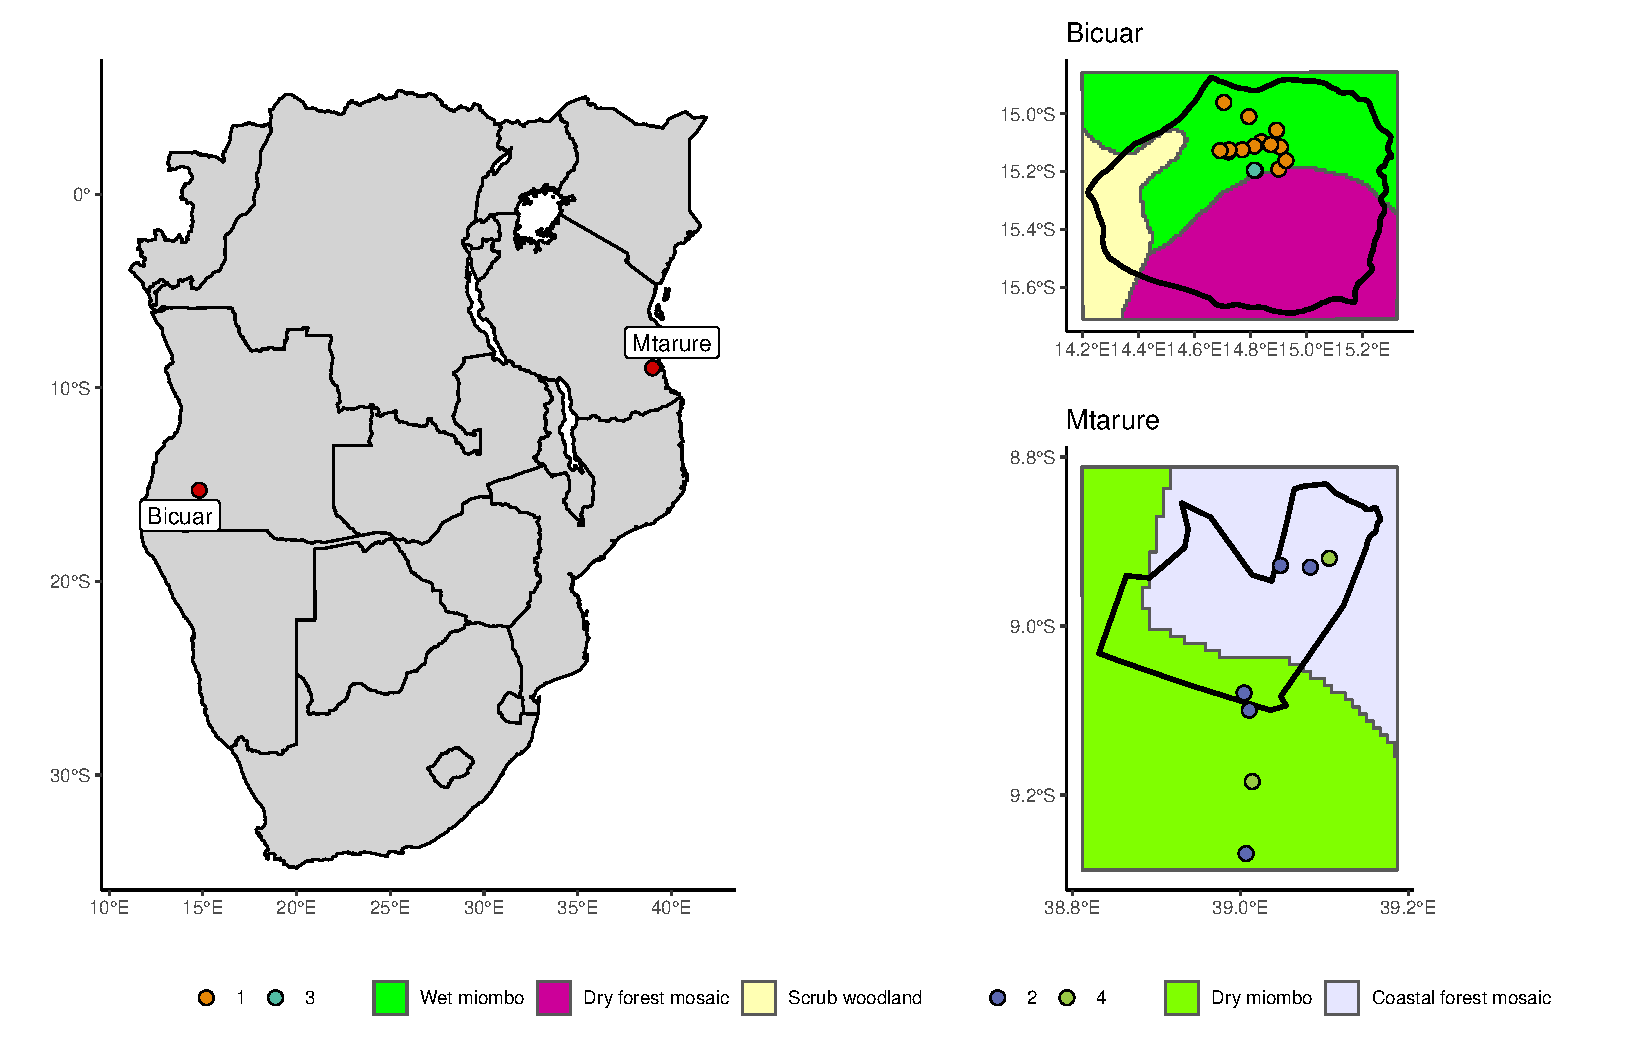
\includegraphics[width=\linewidth]{map}
	\caption{Location of study sites within southern Africa (left), and of 1 ha plots within each site (right). The black outlines in each site map denote the boundaries of protected areas which encompass the majority of study sites, Bicuar National Park in Angola (top), and Mtarure Forest Reserve in Tanzania (bottom). The background of each site map is a re-classified version of White's vegetation map \citep{White1983}. Note that all maps are on different scales.}
	\label{map}
\end{figure}

\subsection{Field measurements}

Within each 1 ha plot each woody stem >5 cm stem diameter was identified to species, the stem diameter was measured (Diameter at Breast Height - 1.3 m) and the stem location within the plot was recorded using tape measures. Each 1 ha plot was further subdivided into nine 10 m diameter circular subplots arranged in a regular grid, with a 15 m buffer from the plot edge and 35 m between subplots. For each subplot, the distance and direction from the subplot centre of each stem >5 cm diameter with canopy material inside the subplot was recorded. Within each subplot, a variable number of scans were recorded using a Leica HDS6100 phase-shift Terrestrial Laser Scanner (TLS). The number and position of scans within a subplot was determined by the arrangement of canopy material in the subplot, to minimise shadows within the canopy of the subplot, and to maximise canopy penetration. The number of scans per subplot ranged between one and five across both sites. Extended field methods and data analysis methods are described in Chapter 6.

\subsection{Data analysis}

\subsubsection{TLS processing}

Point clouds from scans in each subplot were registered and unified using Leica Cyclone (version 9.1), using five reflective cross targets visible to all scans. Point clouds were voxelised to cubic voxels of different sizes depending on the application of the data. Subplot height profile estimation and gap fraction was conducted using 5 cm\textsuperscript{3} voxels, while whole plot canopy rugosity was estimated using 50 cm\textsuperscript{3} voxels. Voxels were classified as `filled' if they intersected one or more points. Variation in voxel size reflects the spatial scale of each analysis, and is bounded by the beam divergence of the scanner over longer distances \citep{Cifuentes2014}. Choosing voxels that are too small can result in pock-marked representations of surfaces that are especially problematic when calculating larger scale canopy structure metrics such as canopy top roughness, while voxels that are too large can result in an over-estimation of plant volume when estimating canopy foliage density at the subplot scale \citep{Seidel2012, Cifuentes2014}. The noise reduction algorithm from \citet{Rusu2008} was used to discard points based on mean nearest neighbour distances, with a mean number of neighbours of eight, and a standard deviation threshold of 1.96. This effectively removed `ghost points' produced by partial beam interceptions and also removed many erroneous returns caused by airborne dust particles, which was common at these study sites. Raw points clouds for each subplot had a mean of \textasciitilde{}\rawpt{} points, \textasciitilde{}\voxelpt{} points after voxelisation to 5 cm\textsuperscript{3}, and \textasciitilde{}\subpt{} points after noise reduction. Ground points were classified using the Progressive Morphological Filter (PMF) from \citet{Zhang2003}. Point cloud height was reclassified height based on this revised ground layer by measuring the vertical distance between the nearest ground point and each point. Points below 1.3 m height above ground were discarded for calculations of foliage density, canopy cover, and foliage complexity, as points below this threshold where often occupied by long grass.

Ray-tracing was used to estimate canopy closure in each subplot, i.e. the proportion of the sky hemisphere occluded by plant material at the subplot centre from multiple TLS scans. Hemispherical images were created using the POV-Ray ray-tracing software \citep{Povray2004}. Filled voxels were represented as matt black cubes filling the voxel volume, with a white sky box and no light source. A `camera' with a 180\textdegree{} fisheye lens was placed at the subplot centre within POV-Ray, at a height of 1.8 m pointing directly upwards. The images produced by POV-Ray were analysed using Hemiphot \citep{HemiPhot} to estimate canopy closure. Canopy closure estimates from the TLS were validated with hemispherical photographs taken at the same location and processed using the same method in Hemiphot, and compared using Pearson's correlation (\hemiCor{}). The Effective Number of Layers (ENL) measures vertical variation in subplot foliage density and was calculated as the true-numbers equivalent Shannon entropy of foliage density among 50 cm layers within each subplot (sensu \citealt{Ehbrecht2016}). Total foliage density was calculated as the area under the curve of the foliage height profile. 

Plot level canopy surface models were extracted using the 99th percentile of canopy height in 10 cm\textsuperscript{2} columns, followed by pit-filling according to \citet{Khosravipour2014} at 50 cm\textsuperscript{2} resolution. Whole plot canopy complexity was measured by two metrics. Canopy top roughness was measured as the standard deviation of canopy height across the plot. Canopy rugosity was measured according to \citet{Hardiman2011}, as the standard deviation of vertical and horizontal foliage density within 0.5 m\textsuperscript{3} cubic bins. Additionally, plot level canopy closure was calculated as the mean of canopy closure values from each subplot.

\subsubsection{Stand structure}

For each subplot, an adapted version of the Iterative Hegyi index was used to estimate crowding, as an alternative to stem density which does not adequately capture crowding at small spatial scales when only a small number of trees are included in the sample \citep{Hegyi1974}. The coefficient of variation of stem diameter was calculated as a measure of the heterogeneity of tree size in the neighbourhood. 

At the plot level, the regularity of species spatial distribution was estimated using the spatial mingling index \citep{Gadow2002}, which scores each tree based on whether it shares species identity with its nearest neighbours. The spatial regularity of trees was estimated using the uniform angle index (winkelmass) \citep{Gadow2002}, which scores each tree based on the angles between nearest neighbours. Additionally, the degree of spatial clustering of trees was measured using Voronoi tessellation, as the coefficient of variation of Voronoi cell areas \citep{Ong2012}. Finally, plot level tree density was calculated to estimate crowding at the plot scale. See Chapter 6 for more information on the behaviour of the spatial mingling index and uniform angle index.

\subsubsection{Statistical analysis}

Non-metric Multi-dimensional Scaling (NMDS) was used to describe variation in species composition among plots, using genus-level basal area weighted abundance in each plot. Stems that could not be identified to genus were excluded from this analysis, which accounted for \perIndet{}\% of the total basal area recorded. Four distinct vegetation types were identified, two from each site (\autoref{clust_summ}). 

Linear mixed effects models tested the effects of tree species diversity and stand structural diversity on subplot canopy complexity metrics. Mixed models used a nested random intercept structure to account for the sampling design of subplots within plots and plots within vegetation types. Separate models were fitted for each canopy complexity metric, resulting in four models at the subplot level. Effect sizes among fixed effects in maximal models were compared for each canopy complexity metric, using the 95\% confidence interval of the effect size to ascertain whether a fixed effect was significant by whether the confidence interval overlapped zero \citep{Nakagawa2007}. AIC values and Akaike weights of models with different combinations of fixed effects were compared to determine which combination of diversity and structural metrics best explained variation in each canopy complexity metric. 

Path analysis was used to test whether tree species diversity may influence canopy complexity indirectly through its effect on stand structure, using the \texttt{piecewiseSEM} R package \citep{piecewiseSEM}. The path analysis investigated the direct effect of plot species richness on mean plot canopy closure, as well as the indirect effect of richness on canopy closure via the coefficient of variation of basal area, with random intercept terms for each vegetation type. The ex-Acacia vegetation type was represented by only two plots and could not be included in this model due to lack of replication.

Statistical analysis of the determinants of plot level canopy complexity metrics were conducted using linear models. Again, these models excluded the ex-Acacia vegetation type due to lack of replication. As with the subplot linear mixed models, predictor variable effect sizes were used to assess predictor variable significance, and comparison of candidate models using AIC, Akaike weights, and model R\\textsuperscript{2} values was used to determine which combination of predictors best explained each canopy complexity metric.

% latex table generated in R 4.1.0 by xtable 1.8-4 package
% Tue Aug 17 09:55:58 2021
\begin{table}[]
\centering
\caption{Description of the vegetation type clusters, identified using the Ward algorithm based on basal area weighted genus abundance. AGB = Above-Ground woody Biomass. Species richness, stem density and AGB are reported as the median among plots, with the interquartile range in parentheses.} 
\label{clust_summ}
\begin{tabular}{lcS[table-format=2.0]rrr}
  \toprule
{Site} & {Cluster} & {N sites} & {Richness} & \thead{Stem density\\(Stems ha\textsuperscript{-1})} & \thead{AGB\\(t ha\textsuperscript{-1})} \\ 
  \midrule
Bicuar & 1 & 12 & 17(2) & 642(194) & 41( 8.4) \\ 
  Mtarure & 2 & 5 & 23(4) & 411(137) & 72(11.9) \\ 
  Bicuar & 3 & 3 &  6(1) & 196( 55) & 77( 7.3) \\ 
  Mtarure & 4 & 2 & 12(2) & 288( 73) &  9( 0.2) \\ 
   \bottomrule
\end{tabular}
\end{table}



% latex table generated in R 4.1.0 by xtable 1.8-4 package
% Mon Aug 23 10:55:27 2021
\begin{table}[]
\centering
\caption{Floristic description of the vegetation type clusters. Dominant species are the most abundant individuals across all plots per cluster. Indicator species are derived from Dufr\^{e}ne-Legendre indicator species analysis with the three highest indicator values.} 
\label{indval}
\begin{tabular}{crrS[table-format=1.2]}
  \toprule
{Cluster} & {Dominant species} & {Indicator species} & {\thead{Indicator\\value}} \\ 
  \midrule
{\multirow{3}{*}{1}} & Julbernardia paniculata & Strychnos spinosa & 0.83 \\ 
   & Burkea africana & Combretum collinum & 0.74 \\ 
   & Combretum collinum & Julbernardia paniculata & 0.70 \\ 
   \midrule
{\multirow{3}{*}{2}} & Diplorhynchus condylocarpon & Pteleopsis myrtifolia & 1.00 \\ 
   & Pseudolachnostylis maprouneifolia & Diplorhynchus condylocarpon & 0.89 \\ 
   & Gymnosporia senegalensis & Pseudolachnostylis maprouneifolia & 0.81 \\ 
   \midrule
{\multirow{3}{*}{3}} & Baikiaea plurijuga & Baikiaea plurijuga & 0.94 \\ 
   & Baphia massaiensis & Baphia massaiensis & 0.83 \\ 
   & Philenoptera nelsii & Philenoptera nelsii & 0.45 \\ 
   \midrule
{\multirow{3}{*}{4}} & Combretum apiculatum & Vachellia nilotica & 0.99 \\ 
   & Burkea africana & Combretum apiculatum & 0.70 \\ 
   & Bauhinia petersiana & Senegalia polyacantha & 0.62 \\ 
   \bottomrule
\end{tabular}
\end{table}



\section{Results}

\subsection{Description of vegetation types}

Indicator species analysis shows that the four identified vegetation types constitute common southern African savanna floristic archetypes (\autoref{indval}). Cluster 1, found in Bicuar National Park contains typical miombo species from the Detarioideae subfamily, such as \textit{Julbernardia paniculata}. Cluster 1 is the most common vegetation type in this study, with 12 plots. Cluster 1 has the highest stem density, but lower AGB than Clusters 2 or 3, which contain larger individuals with disproportionately higher biomass. Cluster 2, found in Mtarure Forest Reserve, is dominated by \textit{Pteleopsis myrtifolia}, a common miombo species from the Combretaceae family. Indeed, Cluster 2 also contained other common miombo species shared with plots in Cluster 1, such as \textit{Julbernardia globiflora} and \textit{Pseudolachnostylis maprouneifolia}, but these clusters remain distinct due to genera endemic to different parts of the miombo ecoregion. Cluster 3 represents \textit{Baikiaea} woodland, found on Kalahari sands in southern Angola. It is species poor and dominated by \textit{Baikiaea plurijuga} which forms large spreading canopy trees with high AGB. Other shrubby species that coppice readily in response to disturbance by fire such as \textit{Baphia massaiensis} are also common. Cluster 4, found in Mtarure is a type of ex-Acacia woodland, dominated by \textit{Vachellia} and \textit{Senegalia} spp. This vegetation type was not well represented in the study, with only two plots, precluding its use in some multi-level statistical analyses due to lack of replication. Cluster 4 had far lower AGB than the other clusters (\autoref{clust_summ}). 

Differences in canopy structure among the four vegetation types are evident through observation of canopy surface models for typical plots within each vegetation type (\autoref{veg_type_tile}). Cluster 1 shows many overlapping crowns forming a nearly contiguous canopy surface. Though most trees in Cluster 1 have smaller crowns than those in Cluster 2, which also forms a nearly contiguous canopy. The largest trees in Cluster 2 grow taller and have a wider spreading canopy than those in other vegetation types. Cluster 3 shows two distinct size classes of tree, the large \textit{Baikiaea plurijuga} forming clear isolated canopies, and much smaller scattered shrubby individuals in the understorey. Cluster 4 shows many small shrubby individuals with irregular canopy shapes, but a greater total crown area coverage than Cluster 3. 

\begin{figure}
	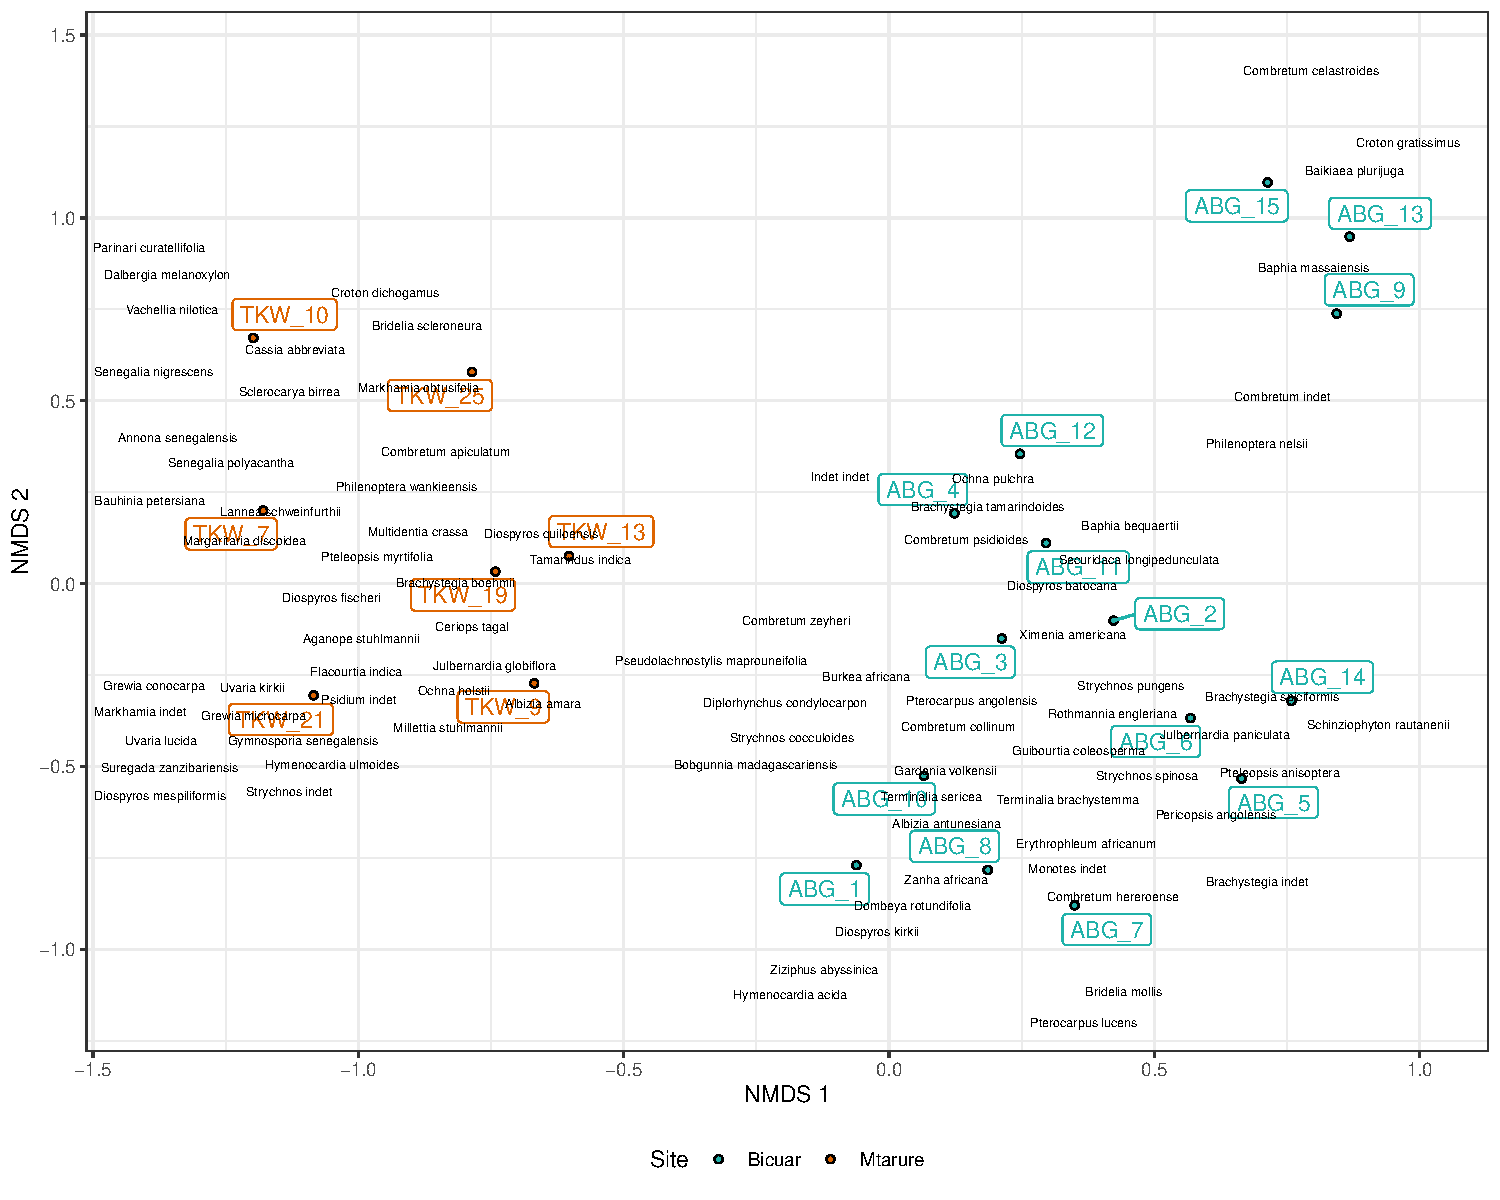
\includegraphics[width=\linewidth]{nmds}
	\caption[NMDS of plots based on genera basal area abundance]{The first two axes of a Non-metric Multi-Dimensional Scaling (NMDS) analysis of tree genus diversity in each plot. Genus scores are labelled as black text, while plot scores are labelled as coloured points. Plots can be split into four principal floristically defined vegetation types: 1) B1-B8, B10-B12, B14, dominated by core miombo species such as \textit{Julbernardia} spp., \textit{Brachystegia} spp.; 2) M2, M5, M6, and M7, also dominated by core miombo genera with some genera not found in Angola to such a great extent such as \textit{Commiphora} and \textit{Sorindeia}; 3) B9, B13 and B15, dominated by \textit{Baikiaea plurijuga}; and 4) M1, M3, and M4, dominated by \textit{Senegalia} spp. and \textit{Vachellia} spp..}
	\label{nmds}
\end{figure}

\subsection{Bivariate relationships}

Bivariate plots and linear models show that subplot species diversity, measured by species richness of the tree neighbourhood around each 10 m diameter subplot, appears to have weak positive effects on subplot canopy layer diversity (\richLayerDiv{}), canopy closure (\richCover{}) and foliage density (\richFoliage{}) (\autoref{subplot_canopy_bivar}). The Hegyi crowding index had strong positive effects on all canopy complexity metrics, as expected. The effect of Hegyi crowding on subplot canopy complexity metrics was similar across all vegetation types. Structural diversity, measured as the coefficient of variation of subplot stem basal area had significant very weak positive effects on total canopy foliage (\baCovFoliage{}) and layer diversity (\baCovLayerDiv{}), but negligible effects on canopy closure (\baCovCover). 

At the plot level, effects of species diversity and stand structure on canopy structure were similarly weak (\autoref{subplot_canopy_bivar}). Spatial clustering of stems, measured by uniform angle index, on canopy closure, was clearly negative (\winkelCoverP{}). Additionally, there was a non-significant negative effect of coefficient of variation of basal area on whole canopy rugosity (\baCovRugosityP{}). Species richness appeared to have strong positive relationships with canopy closure and canopy height, and negative effects on canopy roughness and canopy rugosity. Linear models were highly leveraged by one particularly speciose plot in Cluster 2, with over 40 species, though when this plot was removed, linear model slopes remained significant and with the same sign. Additionally, Cluster 4 represented an outlier in plot level bivariate relationships, with very low canopy closure, and low canopy height, as well as low species richness and low variation in stem size.

\begin{landscape}
\begin{figure}
	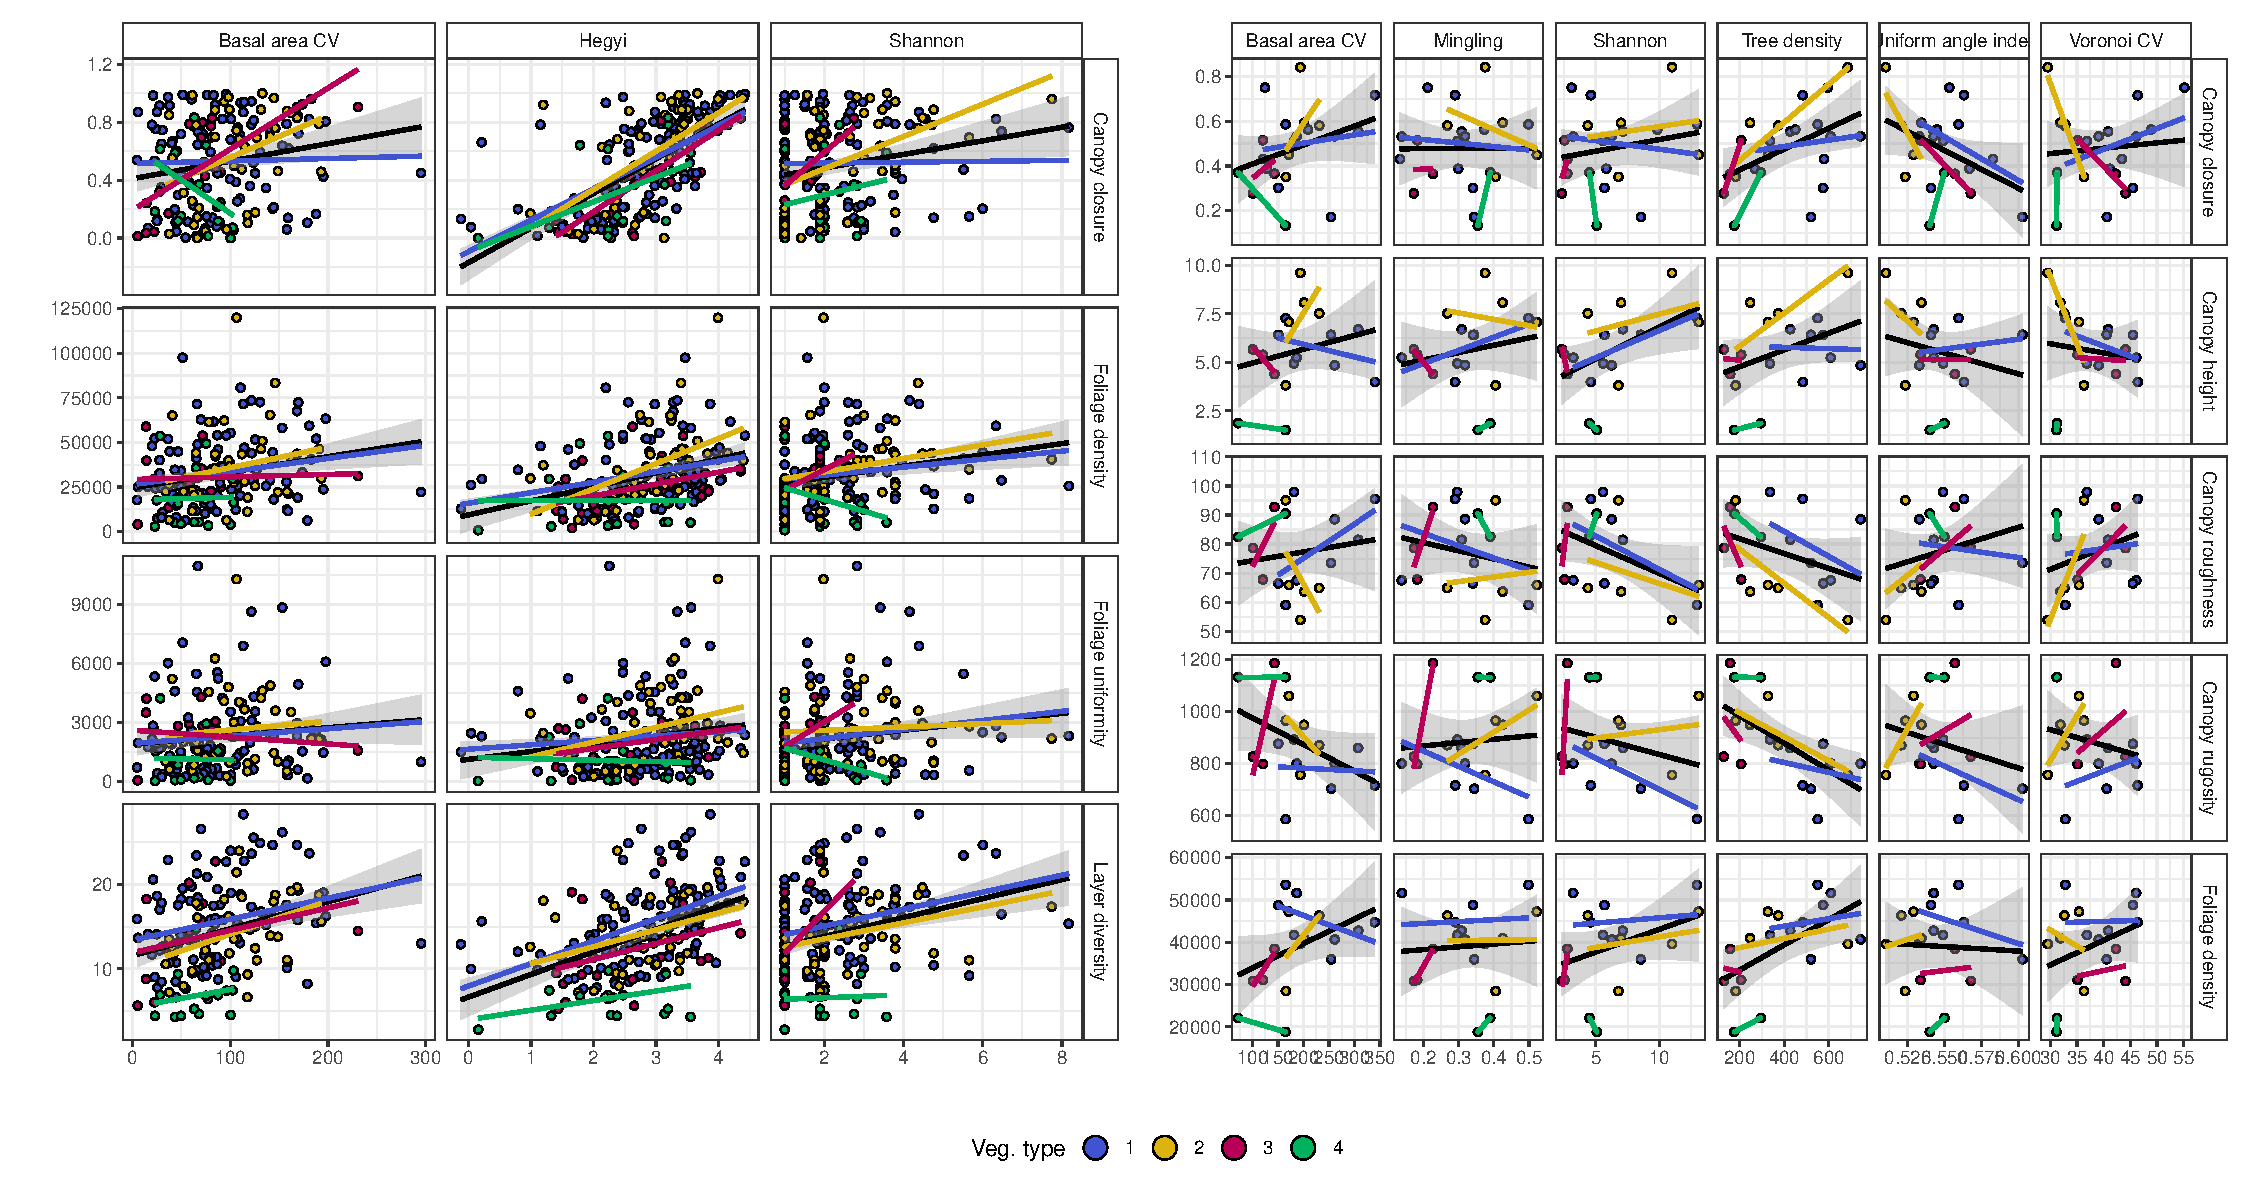
\includegraphics[width=\linewidth]{bivar}
	\caption[Bivariate plots comparing diversity, stand structure and canopy structure]{Bivariate relationships between diversity/stand structure metrics (x axis) and canopy structure metrics (y axis), at both the subplot level (left) and the plot level (right). Points and linear model lines of best fit are coloured by vegetation type. Black lines of best fit are linear models including all plots, with a 95\% confidence interval. See \autoref{bivar_lm_summ} for a comparison of linear model fits by vegetation type.}
	\label{subplot_canopy_bivar}
\end{figure}
\end{landscape}

\begin{figure}
	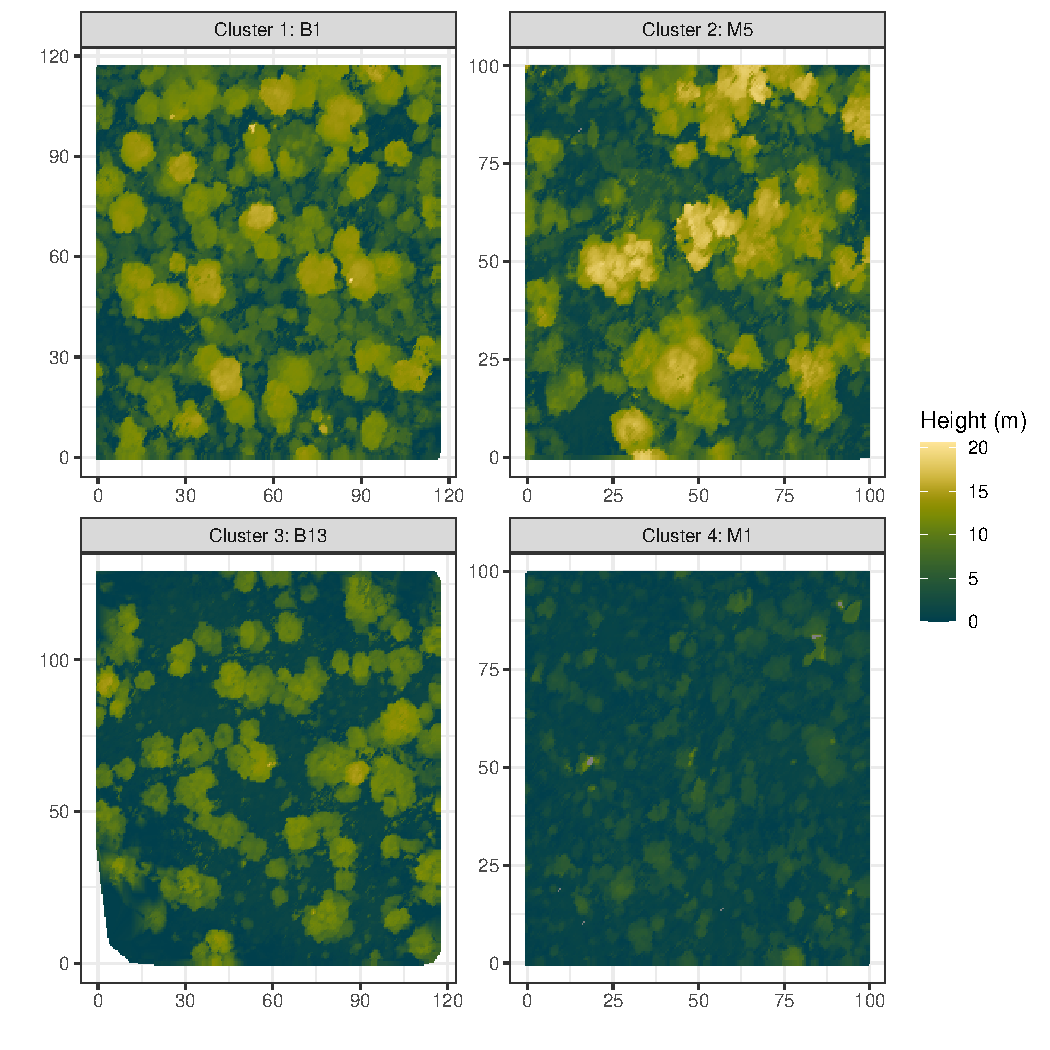
\includegraphics[width=\linewidth]{veg_type_tile}
	\caption{Representative canopy surface models for each vegetation type identified in the Non-metric Multi-dimensional Scaling (NMDS) analysis. Panel titles show the plot name and the vegetation type.}
	\label{veg_type_tile}
\end{figure}

\subsection{Subplot mixed models}

Linear mixed effects models showed that species richness of the subplot neighbourhood had negligible and poorly constrained effects on canopy structure (\autoref{height_profile_mod_rich_slopes_sites}). As seen in the subplot bivariate relationships \autoref{subplot_canopy_bivar}, the Hegyi crowding index had strong positive effects on all measured canopy complexity metrics, though these effects were non-significant for vegetation clusters 3 and 4. Heterogeneity of stem basal area had a significant positive effect on layer diversity, but there was wide variation in vegetation type marginal effects for Clusters 3 and 4, due to low levels of replication. Cluster 3 had a significant positive effect of species richness on foliage distribution uniformity, while none of the other vegetation clusters did.

\begin{figure}
	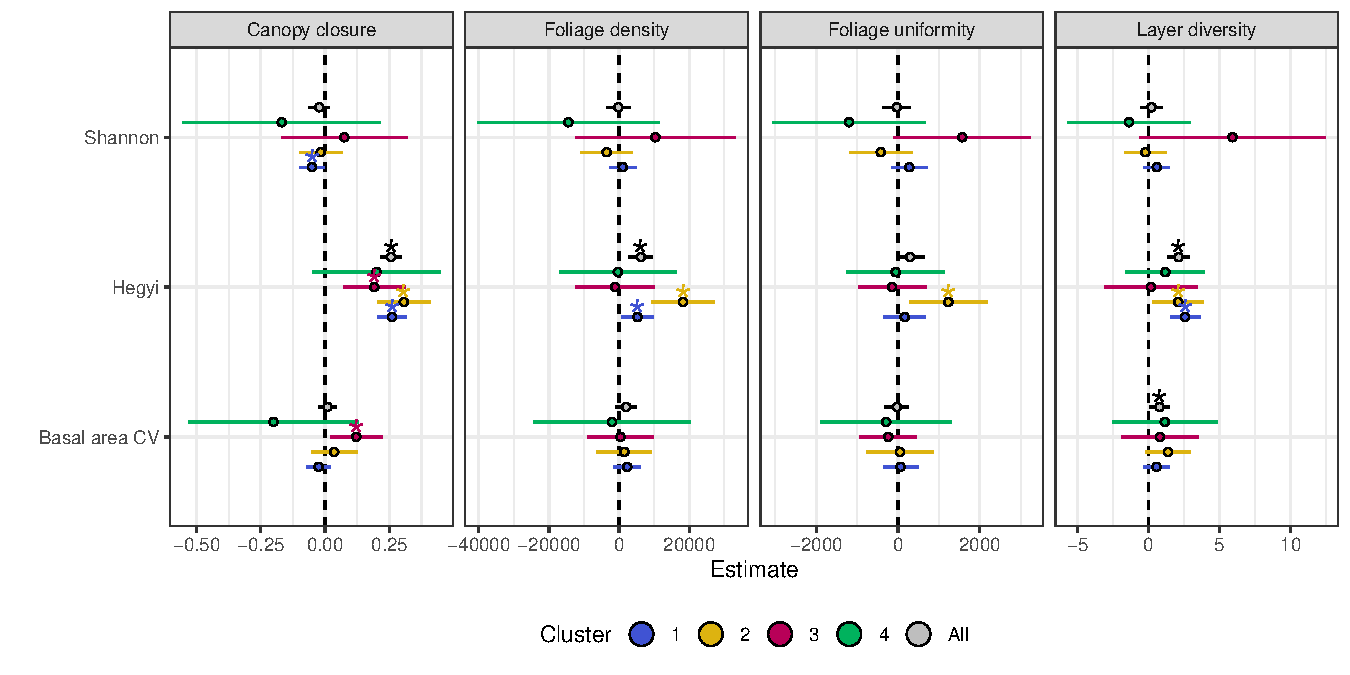
\includegraphics[width=\linewidth]{height_profile_mod_rich_slopes_sites}
	\caption{Standardized fixed effect slopes for each model of a canopy structure metric. Slope estimates where the interval ($\pm$1 standard error) does not overlap zero are considered to be significant effects, marked with asterisks. Points are coloured according to vegetation type.}
	\label{height_profile_mod_rich_slopes_sites}
\end{figure}

Model selection showed that none of the best models for subplot canopy complexity metrics included species richness (\autoref{height_profile_sig_vars_dredge}). The coefficient of variation of basal area was included in the best models for layer diversity and foliage density, with the fixed effects for these models explaining \bestLayerDivRsqS\% and \bestDensRsqS\% of the variation in these metrics, respectively. The random effects of vegetation type and plot identity described most of the variation in layer diversity and foliage density. All models were better than random effects only models according to AIC values.

% latex table generated in R 4.1.0 by xtable 1.8-4 package
% Tue Aug 17 10:02:04 2021
\begin{table}[]
\centering
\caption{Explanatory variables included in the best model for each canopy structure variable. $\Delta$AIC shows the difference in model AIC value compared to a null model which included only the hegyi crowding index and the random effects of vegetation type and plot. R\textsuperscript{2}\textsubscript{c} is the R\textsuperscript{2} of the best model, while R\textsuperscript{2}\textsubscript{m} is the R\textsuperscript{2} of the model fixed effects only.} 
\label{height_profile_sig_vars_dredge}
\begin{tabular}{lcccccc}
  \toprule
{Response} & {Hegyi} & {Richness} & {\thead{Basal area\\CoV}} & {$\Delta$AIC} & {R\textsuperscript{2}\textsubscript{c}} & {R\textsuperscript{2}\textsubscript{m}} \\ 
  \midrule
Layer diversity & \checkmark &  & \checkmark & 37.4 & 0.50 & 0.17 \\ 
  Foliage density & \checkmark &  &  & 62.4 & 0.27 & 0.09 \\ 
  Canopy closure & \checkmark &  &  & 93.9 & 0.60 & 0.46 \\ 
   \bottomrule
\end{tabular}
\end{table}



\subsection{Whole-plot multivariate linear models}

While species diversity had varying effects on different plot level canopy complexity metrics, the confidence intervals on these effect sizes were wide (\autoref{canopy_rough_slopes}). Species richness had a significant positive effect on canopy height (\richHeightP{}), a non-significant positive effect on canopy closure (\richCoverP{}), but a negative effect on canopy surface roughness (\richRoughP{}). Plot tree density had negligible effects on canopy complexity, except for canopy rugosity (\treeDensRugP{}), in contrast to the effect of Hegyi crowding on subplot canopy complexity. Structural diversity, measured by the coefficient of variation of basal area had a positive effect on canopy roughness (\covBARoughP{}). Spatially explicit measures of structural and species diversity, measured by the uniform angle index and spatial mingling index respectively, had negligible effects on all canopy complexity metrics. One exception was the effect of uniform angle index, i.e. the spatial clustering of stems, on canopy closure, which was clearly negative (\wiCoverP{}). 

Despite the weak effect sizes of species richness on canopy complexity at the plot level, model selection showed that canopy height, canopy roughness, and canopy closure were better explained by models which included species richness (\autoref{canopy_sig_vars_dredge}). Additionally, the best model for canopy closure included spatial clustering of trees. Though the model for canopy roughness was only marginally better than a null model, and had a non-significant p-value. Canopy rugosity was poorly predicted by all candidate models.

\begin{figure}
	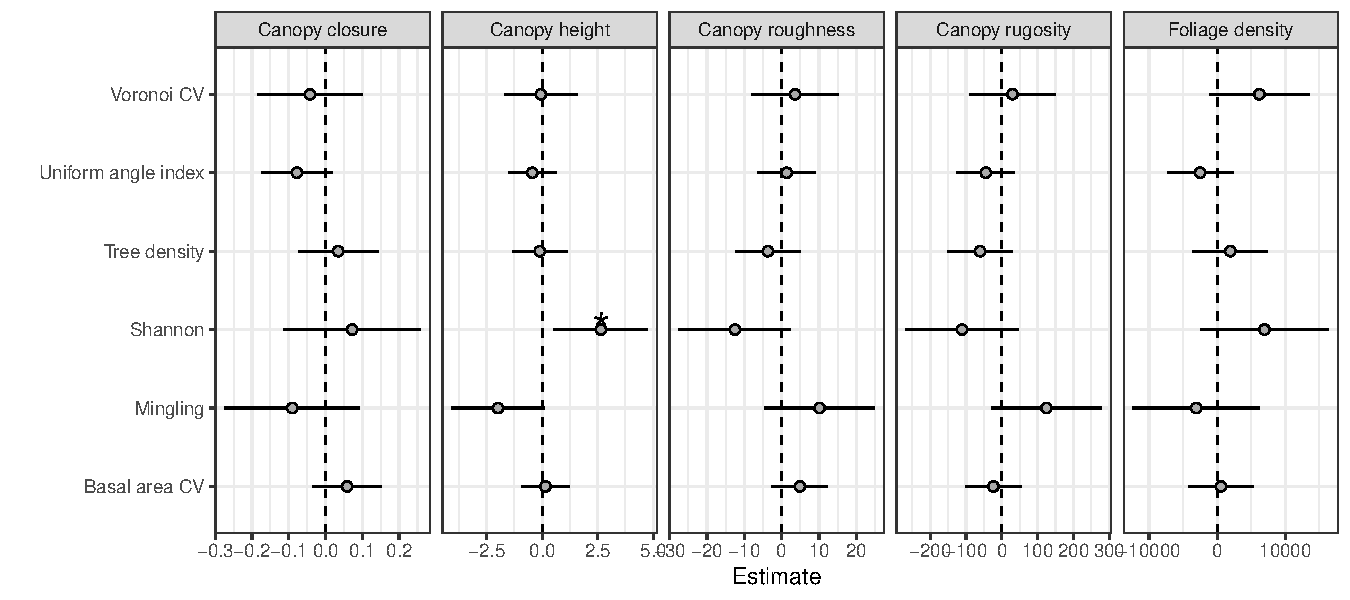
\includegraphics[width=\linewidth]{canopy_rough_slopes}
	\caption{Standardized effect sizes for whole-plot canopy rugosity. Slope estimates where the interval ($\pm$1 standard error) does not overlap zero are considered to be significant effects, marked with asterisks.}
	\label{canopy_rough_slopes}
\end{figure}


% latex table generated in R 4.1.0 by xtable 1.8-4 package
% Sat Aug 21 08:31:10 2021
\begin{table}[ht]
\centering
\caption{Explanatory variables included in the best linear model for each plot-level canopy complexity metric. $\Delta$AIC shows the difference in model AIC value compared to a null model.} 
\label{canopy_sig_vars_dredge}
\setlength{\tabcolsep}{4pt}
\begin{tabular}{lccccccccS[table-format=<1.2]}
  \toprule
{Response} & {Richness} & {\thead{Tree\\density}} & {\thead{Basal area\\CoV}} & {Mingling} & {\thead{Uniform\\angle index}} & {\thead{Voronoi\\CoV}} & {$\Delta$AIC} & {R\textsuperscript{2}} & {Prob.} \\ 
  \midrule
Foliage density & \checkmark &  &  &  &  & \checkmark & 2.7 & 0.56 & 0.11 \\ 
  Canopy closure & \checkmark &  &  &  &  &  & 2.8 & 0.56 & 0.1 \\ 
  Canopy height & \checkmark &  &  &  &  &  & 0.9 & 0.51 & 0.17 \\ 
  Canopy roughness & \checkmark &  & \checkmark &  &  &  & 0.6 & 0.50 & 0.18 \\ 
  Canopy rugosity &  & \checkmark &  &  &  &  & 1.0 & 0.51 & 0.16 \\ 
   \bottomrule
\end{tabular}
\end{table}



\subsection{Path analysis}

The path analysis investigating the indirect effect of subplot species richness on canopy closure via the coefficient of variation of basal area showed that while species richness had a strong positive significant effect on basal area variation, the effect of basal area variation on canopy closure remained negligible (\autoref{path_diag}). The indirect effect of species richness on canopy closure via basal area coefficient of variation was \ccind{}, while the direct effect was \ccdir{}. As in the bivariate relationships and plot level linear models, species richness had a weak positive significant effect on canopy closure, while the major driver of canopy closure was the Hegyi crowding index.

\begin{figure}
	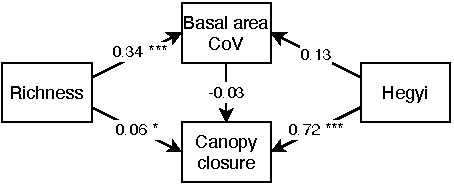
\includegraphics[width=0.8\linewidth]{path_diag}
	\caption{Directed Acyclic Graph showing path coefficients for the path analysis of the indirect effect of species richness on canopy closure via coefficient of variation of basal area. Paths are labelled according to their standardized path coefficient. Asterisks define p-value thresholds: *<0.05, **<0.01, ***<0.001.}
	\label{path_diag}
\end{figure}



\subsection{Comparing subplot and plot measures of canopy structure}

Plot and subplot canopy structure metrics were highly correlated in many cases, with similar relationships among vegetation types (\autoref{canopy_rough_slopes}). Most subplot and plot level canopy metrics covaried in a predictable manner. For example, increased canopy height led to an increase in canopy closure. Plot canopy height especially, tended to be strongly positively correlated with subplot canopy complexity metrics. Additionally, as canopy rugosity increased, many subplot canopy complexity and density metrics decreased. Subplot metrics varied greatly within plots, producing large uncertainty in plot level estimates of these metrics. 

\begin{figure}
	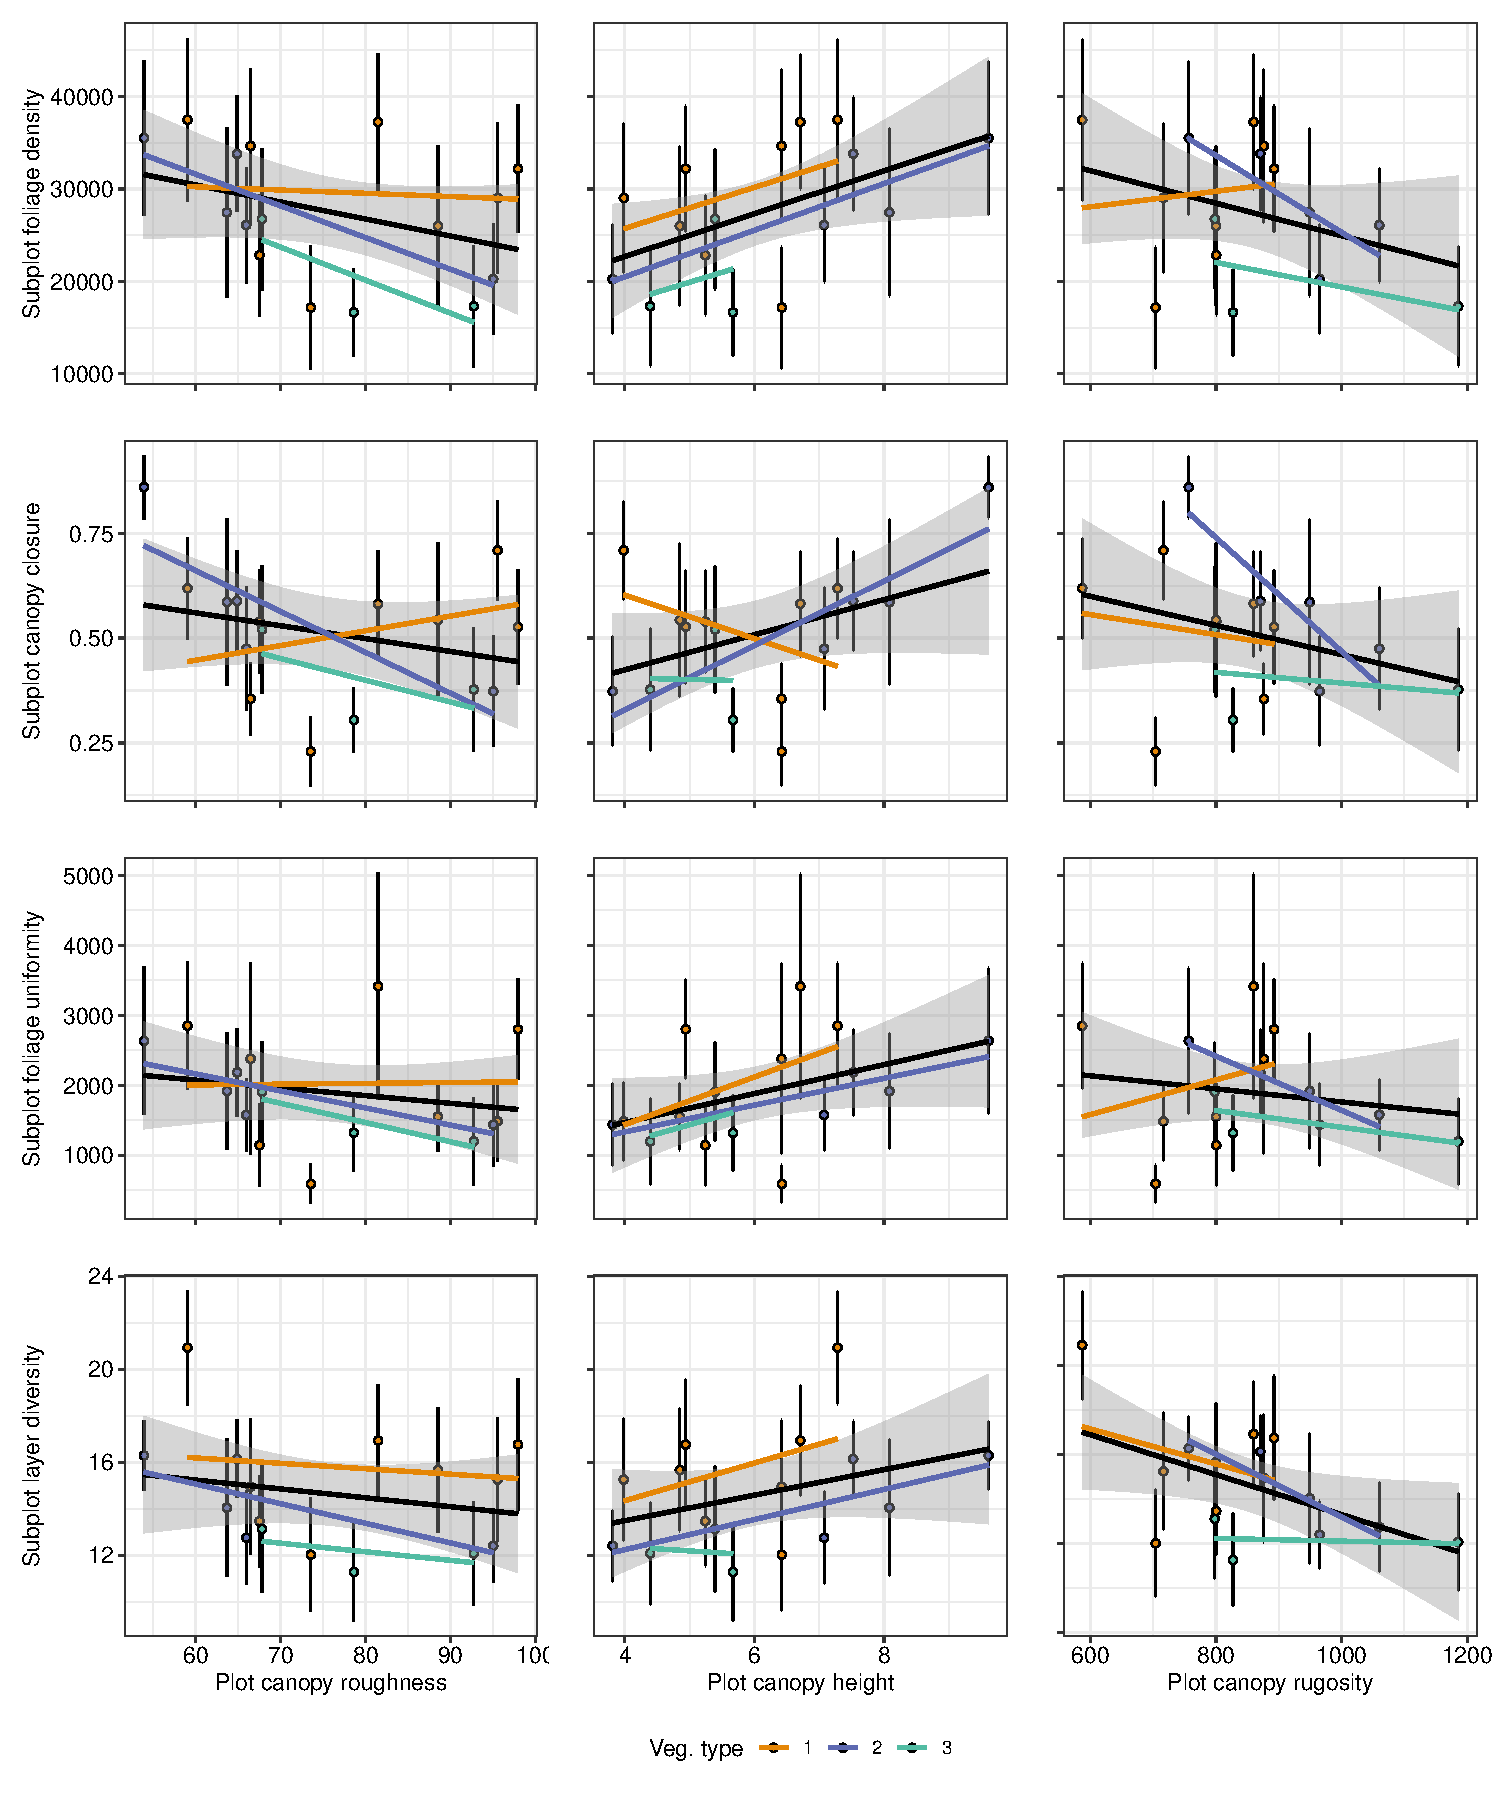
\includegraphics[width=\linewidth]{plot_subplot_bivar}
	\caption{Bivariate plots comparing canopy structural metrics at the plot (x axis) and subplot scale (y axis). Each point represents the mean values of a single plot. Points and linear model fits are coloured according to vegetation type. The black linear model combines all vegetation types. Error bars on points are the standard deviation of mean subplot metrics across the plot.}
	\label{plot_subplot_bivar}
\end{figure}

\section{Discussion}

This study investigated relationships between tree species diversity, stand structure, and several metrics of tree canopy complexity using terrestrial LiDAR in southern African savannas, with a view to improving understanding of the biotic drivers of variation in canopy structure and vegetation dynamics. Species diversity, measured by species richness, appeared to generally have weak positive effects on canopy complexity metrics at both the subplot and plot scales. Plots with greater species richness produced taller tree canopies, with a more complex within-canopy structure, and greater canopy closure. However, inherent variability in canopy structure among and within plots makes it difficult to conclusively infer a generalisable species diversity effect across all plots. 

Plot level canopy complexity metrics were generally better predicted by species diversity and stand structure than subplot metrics. While positive relationships between species richness and subplot canopy complexity metrics were observed in the subplot bivariate models, subplot linear mixed effects models did not show strong species richness effects. Additionally, none of the best models for subplot canopy complexity metrics included species richness as a fixed effect. This finding suggests a large degree of stochastic variability in canopy structure within plots, that masks species effects at smaller spatial scales. The prevalence of disturbance events such as fire and damage by elephants in southern African woodlands, as well as tree-fall, small-scale variability in edaphic factors, and stochastic tree germination all contribute to heterogeneity in canopy structure \citep{}. This study demonstrates the importance of large sample units and a high degree of replication when measuring canopy structure, especially in disturbed systems, to effectively account for the inherent heterogeneity in the system \citep{}.
 
Spatial clustering of stems, measured using the uniform angle index, caused a clear decrease in canopy closure, with similar behaviour across vegetation types. Uniform angle index was also included in the best multivariate model predicting canopy closure. This finding is expected, as spatial clustering results in reduced canopy cover in areas outside clusters, and a non-compensatory increase in canopy closure within clusters, due to competition among individuals \citep{}. Clustering of trees in savannas can result from positive feedback effects from disturbance by fire and herbivory \citep{}. This study suggests that as well as reducing canopy cover, i.e. the ground area covered by tree canopies, disturbances in savannas may also serve to decrease canopy closure, i.e. the visible sky proportion from both within canopy gaps and between canopy gaps, indirectly by increasing spatial clustering of trees. The negative effects of spatial clustering on canopy closure are expected to increase in species poor woodlands, due to a lack of niche complementarity among coexisting individuals \citep{}. 

Stand structural diversity caused positive canopy complexity effects for within-canopy structural metrics such as layer diversity and canopy surface roughness, but had negligible effects on canopy density. This is in line with other studies in forest ecosystems, which report that variation in tree size increases total canopy volume occupancy by increasing the number of canopy layers, but does not necessarily result in a concomitant increase in canopy closure, as the resulting canopies are often more sparse, especially for understorey individuals \citep{}. The path analysis also supports this conclusion, where species richness was found to cause an increase in stand structural diversity, but this did not extend to an increase in canopy closure. 

The effect of stand structure on canopy complexity in this system appears to be a result of demographic effects rather than variation in growth form as a function of species diversity. The path analysis testing the indirect effect of species diversity on canopy closure via stand structural diversity did not find a significant indirect effect of species diversity on canopy closure. While other studies in forests have found a species diversity effect on stand structural diversity \citep{}, it is suggested here that prevailing disturbance pressures mask any species diversity effect.

Effects of species composition, measured by vegetation type, on canopy structure were small. While vegetation types differed in mean values for stand structural and species diversity metrics, variation in these metrics produced results of similar direction and magnitude among vegetation types in most cases. Small sample sizes for \textit{Baikiaea} and ex-Acacia vegetation however, led to wide errors on most relationships especially at the plot level, such that it is impossible to draw deeper conclusions about the behaviour of these vegetation types. Variation in mean values of canopy complexity metrics among vegetation types is likely driven by species identity \citep{}, though species composition itself is likely driven by environmental factors and disturbance regime \citep{}. 


\section{Conclusion}

\printbibliography

%\section{Supplementary Material} \beginsupplement

% latex table generated in R 4.1.0 by xtable 1.8-4 package
% Sat Aug 21 16:12:18 2021
\setlength{\tabcolsep}{4pt}
\begin{longtable}{llccccS[table-format=-2.2, table-space-text-post = {***}]}
\caption{Summary statistics of bivariate linear models comparing canopy complexity metrics with diversity and stand structural metrics. Slope refers to the slope of the predictor term in the model, $\pm{}$ 1 standard error. R\textsuperscript{2} refers to the whole model. T is the t-value of the slope of the predictor term in the model, Asterisks indicate the p-value of these terms (***<0.001, **<0.01, *<0.05).} \\ 
  \toprule
{Response} & {Predictor} & {Cluster} & {Slope} & {F} & {R\textsuperscript{2}} & {T} \\ 
  \midrule
{\multirow{5}{*}{Foliage density}} & {\multirow{5}{*}{Basal area CV}} & 1 &  7.3e+01$\pm$3.7e+01 & 4.0(2,97) & 0.04 & 1.99* \\ 
   &  & 2 &  1.1e+02$\pm$7.9e+01 & 2.1(2,38) & 0.05 & 1.44 \\ 
   &  & 3 &  1.4e+01$\pm$7.2e+01 & 0.0(2,14) & 0.00 & 0.20 \\ 
   &  & 4 &  1.6e+01$\pm$2.0e+02 & 0.0(2,12) & 0.00 & 0.08 \\ 
   &  & All &  8.7e+01$\pm$3.0e+01 & 8.6(2,167) & 0.05 & 2.93** \\ 
   \midrule
{\multirow{5}{*}{Foliage density}} & {\multirow{5}{*}{Hegyi}} & 1 &  5.9e+03$\pm$2.1e+03 & 8.2(2,102) & 0.07 & 2.86** \\ 
   &  & 2 &  1.4e+04$\pm$3.6e+03 & 15.2(2,40) & 0.28 & 3.90*** \\ 
   &  & 3 &  6.6e+03$\pm$3.0e+03 & 4.8(2,23) & 0.17 & 2.18* \\ 
   &  & 4 &  1.5e+01$\pm$5.5e+03 & 0.0(2,13) & 0.00 & 0.00 \\ 
   &  & All &  7.8e+03$\pm$1.6e+03 & 25.5(2,184) & 0.12 & 5.05*** \\ 
   \midrule
{\multirow{5}{*}{Foliage density}} & {\multirow{5}{*}{Shannon}} & 1 &  2.2e+03$\pm$1.3e+03 & 2.8(2,102) & 0.03 & 1.67 \\ 
   &  & 2 &  3.8e+03$\pm$2.4e+03 & 2.6(2,39) & 0.06 & 1.61 \\ 
   &  & 3 &  1.1e+04$\pm$6.5e+03 & 3.1(2,20) & 0.13 & 1.77 \\ 
   &  & 4 & -6.5e+03$\pm$6.5e+03 & 1.0(2,13) & 0.07 & -1.01 \\ 
   &  & All &  3.2e+03$\pm$1.1e+03 & 8.9(2,180) & 0.05 & 2.98** \\ 
   \midrule
{\multirow{5}{*}{Canopy closure}} & {\multirow{5}{*}{Basal area CV}} & 1 &  1.7e-04$\pm$6.0e-04 & 0.1(2,97) & 0.00 & 0.28 \\ 
   &  & 2 &  2.9e-03$\pm$1.1e-03 & 6.9(2,39) & 0.15 & 2.62* \\ 
   &  & 3 &  4.2e-03$\pm$1.1e-03 & 15.1(2,14) & 0.52 & 3.89** \\ 
   &  & 4 & -4.6e-03$\pm$3.0e-03 & 2.2(2,12) & 0.16 & -1.50 \\ 
   &  & All &  1.2e-03$\pm$4.8e-04 & 6.3(2,168) & 0.04 & 2.52* \\ 
   \midrule
{\multirow{5}{*}{Canopy closure}} & {\multirow{5}{*}{Hegyi}} & 1 &  2.2e-01$\pm$2.8e-02 & 62.3(2,102) & 0.38 & 7.89*** \\ 
   &  & 2 &  2.6e-01$\pm$5.1e-02 & 27.0(2,41) & 0.40 & 5.19*** \\ 
   &  & 3 &  2.8e-01$\pm$4.0e-02 & 50.7(2,23) & 0.69 & 7.12*** \\ 
   &  & 4 &  1.7e-01$\pm$8.0e-02 & 4.5(2,13) & 0.26 & 2.12 \\ 
   &  & All &  2.4e-01$\pm$2.1e-02 & 132.8(2,185) & 0.42 & 11.52*** \\ 
   \midrule
{\multirow{5}{*}{Canopy closure}} & {\multirow{5}{*}{Shannon}} & 1 &  3.1e-03$\pm$2.2e-02 & 0.0(2,102) & 0.00 & 0.14 \\ 
   &  & 2 &  1.1e-01$\pm$3.2e-02 & 12.1(2,40) & 0.23 & 3.48** \\ 
   &  & 3 &  2.3e-01$\pm$1.4e-01 & 2.9(2,20) & 0.13 & 1.69 \\ 
   &  & 4 &  6.7e-02$\pm$1.1e-01 & 0.4(2,13) & 0.03 & 0.60 \\ 
   &  & All &  4.7e-02$\pm$1.7e-02 & 7.3(2,181) & 0.04 & 2.70** \\ 
   \midrule
{\multirow{5}{*}{Foliage uniformity}} & {\multirow{5}{*}{Basal area CV}} & 1 &  3.7e+00$\pm$4.0e+00 & 0.9(2,97) & 0.01 & 0.92 \\ 
   &  & 2 &  4.5e+00$\pm$7.4e+00 & 0.4(2,38) & 0.01 & 0.61 \\ 
   &  & 3 & -3.5e+00$\pm$5.9e+00 & 0.4(2,14) & 0.02 & -0.59 \\ 
   &  & 4 & -9.3e-01$\pm$1.5e+01 & 0.0(2,12) & 0.00 & -0.06 \\ 
   &  & All &  4.1e+00$\pm$3.0e+00 & 1.9(2,167) & 0.01 & 1.37 \\ 
   \midrule
{\multirow{5}{*}{Foliage uniformity}} & {\multirow{5}{*}{Hegyi}} & 1 &  2.2e+02$\pm$2.3e+02 & 1.0(2,102) & 0.01 & 0.98 \\ 
   &  & 2 &  7.5e+02$\pm$3.7e+02 & 4.0(2,40) & 0.09 & 2.00 \\ 
   &  & 3 &  4.5e+02$\pm$2.6e+02 & 2.9(2,23) & 0.11 & 1.72 \\ 
   &  & 4 & -7.5e+01$\pm$4.0e+02 & 0.0(2,13) & 0.00 & -0.19 \\ 
   &  & All &  4.0e+02$\pm$1.6e+02 & 6.2(2,184) & 0.03 & 2.49* \\ 
   \midrule
{\multirow{5}{*}{Foliage uniformity}} & {\multirow{5}{*}{Shannon}} & 1 &  2.3e+02$\pm$1.4e+02 & 2.6(2,102) & 0.02 & 1.61 \\ 
   &  & 2 &  8.6e+01$\pm$2.2e+02 & 0.1(2,39) & 0.00 & 0.38 \\ 
   &  & 3 &  1.3e+03$\pm$5.1e+02 & 6.1(2,20) & 0.23 & 2.48* \\ 
   &  & 4 & -5.9e+02$\pm$4.7e+02 & 1.6(2,13) & 0.11 & -1.27 \\ 
   &  & All &  2.2e+02$\pm$1.1e+02 & 4.1(2,180) & 0.02 & 2.04* \\ 
   \midrule
{\multirow{5}{*}{Layer diversity}} & {\multirow{5}{*}{Basal area CV}} & 1 &  2.5e-02$\pm$9.3e-03 & 7.1(2,97) & 0.07 & 2.66** \\ 
   &  & 2 &  3.9e-02$\pm$1.4e-02 & 8.0(2,38) & 0.17 & 2.83** \\ 
   &  & 3 &  2.7e-02$\pm$2.3e-02 & 1.3(2,14) & 0.09 & 1.15 \\ 
   &  & 4 &  2.1e-02$\pm$3.1e-02 & 0.5(2,12) & 0.04 & 0.67 \\ 
   &  & All &  3.2e-02$\pm$7.6e-03 & 17.6(2,167) & 0.10 & 4.20*** \\ 
   \midrule
{\multirow{5}{*}{Layer diversity}} & {\multirow{5}{*}{Hegyi}} & 1 &  2.7e+00$\pm$4.9e-01 & 29.1(2,102) & 0.22 & 5.39*** \\ 
   &  & 2 &  2.0e+00$\pm$7.5e-01 & 7.1(2,40) & 0.15 & 2.66* \\ 
   &  & 3 &  1.9e+00$\pm$1.0e+00 & 3.6(2,23) & 0.13 & 1.89 \\ 
   &  & 4 &  1.1e+00$\pm$8.5e-01 & 1.8(2,13) & 0.12 & 1.33 \\ 
   &  & All &  2.7e+00$\pm$3.9e-01 & 46.8(2,184) & 0.20 & 6.84*** \\ 
   \midrule
{\multirow{5}{*}{Layer diversity}} & {\multirow{5}{*}{Shannon}} & 1 &  1.0e+00$\pm$3.4e-01 & 8.7(2,102) & 0.08 & 2.95** \\ 
   &  & 2 &  9.5e-01$\pm$4.3e-01 & 4.8(2,39) & 0.11 & 2.18* \\ 
   &  & 3 &  4.9e+00$\pm$1.8e+00 & 7.2(2,20) & 0.26 & 2.68* \\ 
   &  & 4 &  1.8e-01$\pm$1.1e+00 & 0.0(2,13) & 0.00 & 0.16 \\ 
   &  & All &  1.1e+00$\pm$2.7e-01 & 16.8(2,180) & 0.09 & 4.10*** \\ 
   \midrule
{\multirow{5}{*}{Canopy roughness}} & {\multirow{5}{*}{Basal area CV}} & 1 &  1.2e-01$\pm$6.9e-02 & 2.9(2,6) & 0.33 & 1.72 \\ 
   &  & 2 & -3.2e-01$\pm$2.9e-01 & 1.2(2,3) & 0.29 & -1.10 \\ 
   &  & 3 &  3.5e-01$\pm$4.7e-01 & 0.6(2,1) & 0.36 & 0.74 \\ 
   &  & 4 &  &  &  &  \\ 
   &  & All &  3.0e-02$\pm$5.0e-02 & 0.4(2,16) & 0.02 & 0.60 \\ 
   \midrule
{\multirow{5}{*}{Canopy roughness}} & {\multirow{5}{*}{Voronoi CV}} & 1 &  2.6e-01$\pm$1.2e+00 & 0.0(2,6) & 0.01 & 0.22 \\ 
   &  & 2 &  4.6e+00$\pm$1.9e+00 & 6.1(2,3) & 0.67 & 2.48 \\ 
   &  & 3 &  1.8e+00$\pm$1.9e+00 & 1.0(2,1) & 0.49 & 0.99 \\ 
   &  & 4 &  &  &  &  \\ 
   &  & All &  7.5e-01$\pm$5.9e-01 & 1.6(2,16) & 0.09 & 1.26 \\ 
   \midrule
{\multirow{5}{*}{Canopy roughness}} & {\multirow{5}{*}{Mingling}} & 1 & -4.2e+01$\pm$5.7e+01 & 0.5(2,6) & 0.08 & -0.74 \\ 
   &  & 2 &  1.6e+01$\pm$9.7e+01 & 0.0(2,3) & 0.01 & 0.17 \\ 
   &  & 3 &  3.5e+02$\pm$2.5e+02 & 2.0(2,1) & 0.67 & 1.42 \\ 
   &  & 4 &  &  &  &  \\ 
   &  & All & -2.8e+01$\pm$3.3e+01 & 0.7(2,16) & 0.04 & -0.86 \\ 
   \midrule
{\multirow{5}{*}{Canopy roughness}} & {\multirow{5}{*}{Tree density}} & 1 & -4.3e-02$\pm$4.5e-02 & 0.9(2,6) & 0.13 & -0.96 \\ 
   &  & 2 & -5.9e-02$\pm$3.1e-02 & 3.6(2,3) & 0.54 & -1.89 \\ 
   &  & 3 & -1.8e-01$\pm$2.6e-01 & 0.5(2,1) & 0.31 & -0.68 \\ 
   &  & 4 &  &  &  &  \\ 
   &  & All & -2.6e-02$\pm$1.7e-02 & 2.3(2,16) & 0.12 & -1.51 \\ 
   \midrule
{\multirow{5}{*}{Canopy roughness}} & {\multirow{5}{*}{Shannon}} & 1 & -2.3e+00$\pm$1.7e+00 & 1.7(2,6) & 0.22 & -1.32 \\ 
   &  & 2 & -1.4e+00$\pm$2.4e+00 & 0.4(2,3) & 0.11 & -0.60 \\ 
   &  & 3 &  3.4e+01$\pm$4.7e+01 & 0.5(2,1) & 0.34 & 0.72 \\ 
   &  & 4 &  &  &  &  \\ 
   &  & All & -1.9e+00$\pm$9.5e-01 & 4.0(2,16) & 0.20 & -2.01 \\ 
   \midrule
{\multirow{5}{*}{Canopy roughness}} & {\multirow{5}{*}{Uniform angle index}} & 1 & -7.4e+01$\pm$2.6e+02 & 0.1(2,6) & 0.01 & -0.28 \\ 
   &  & 2 &  4.1e+02$\pm$9.5e+02 & 0.2(2,3) & 0.06 & 0.43 \\ 
   &  & 3 &  4.4e+02$\pm$5.7e+02 & 0.6(2,1) & 0.37 & 0.76 \\ 
   &  & 4 &  &  &  &  \\ 
   &  & All &  1.6e+02$\pm$1.6e+02 & 1.0(2,16) & 0.06 & 0.98 \\ 
   \midrule
{\multirow{5}{*}{Canopy height}} & {\multirow{5}{*}{Basal area CV}} & 1 & -6.5e-03$\pm$6.1e-03 & 1.1(2,6) & 0.16 & -1.07 \\ 
   &  & 2 &  4.3e-02$\pm$4.0e-02 & 1.2(2,3) & 0.28 & 1.08 \\ 
   &  & 3 & -3.1e-02$\pm$8.7e-03 & 12.3(2,1) & 0.92 & -3.51 \\ 
   &  & 4 &  &  &  &  \\ 
   &  & All &  7.1e-03$\pm$7.3e-03 & 0.9(2,16) & 0.06 & 0.97 \\ 
   \midrule
{\multirow{5}{*}{Canopy height}} & {\multirow{5}{*}{Voronoi CV}} & 1 & -1.0e-01$\pm$8.6e-02 & 1.5(2,6) & 0.20 & -1.21 \\ 
   &  & 2 & -7.0e-01$\pm$2.0e-01 & 12.7(2,3) & 0.81 & -3.57* \\ 
   &  & 3 & -1.8e-02$\pm$1.4e-01 & 0.0(2,1) & 0.02 & -0.13 \\ 
   &  & 4 &  &  &  &  \\ 
   &  & All & -4.7e-02$\pm$9.1e-02 & 0.3(2,16) & 0.02 & -0.52 \\ 
   \midrule
{\multirow{5}{*}{Canopy height}} & {\multirow{5}{*}{Mingling}} & 1 &  6.8e+00$\pm$3.8e+00 & 3.2(2,6) & 0.34 & 1.78 \\ 
   &  & 2 & -3.3e+00$\pm$1.3e+01 & 0.1(2,3) & 0.02 & -0.25 \\ 
   &  & 3 & -2.3e+01$\pm$9.3e-01 & 619.2(2,1) & 1.00 & -24.88* \\ 
   &  & 4 &  &  &  &  \\ 
   &  & All &  3.8e+00$\pm$4.8e+00 & 0.6(2,16) & 0.04 & 0.79 \\ 
   \midrule
{\multirow{5}{*}{Canopy height}} & {\multirow{5}{*}{Tree density}} & 1 & -3.5e-04$\pm$3.8e-03 & 0.0(2,6) & 0.00 & -0.09 \\ 
   &  & 2 &  8.6e-03$\pm$4.0e-03 & 4.7(2,3) & 0.61 & 2.16 \\ 
   &  & 3 & -1.0e-03$\pm$1.7e-02 & 0.0(2,1) & 0.00 & -0.06 \\ 
   &  & 4 &  &  &  &  \\ 
   &  & All &  4.3e-03$\pm$2.5e-03 & 3.1(2,16) & 0.16 & 1.76 \\ 
   \midrule
{\multirow{5}{*}{Canopy height}} & {\multirow{5}{*}{Shannon}} & 1 &  2.8e-01$\pm$1.1e-01 & 7.1(2,6) & 0.54 & 2.66* \\ 
   &  & 2 &  1.7e-01$\pm$3.3e-01 & 0.3(2,3) & 0.08 & 0.52 \\ 
   &  & 3 & -3.0e+00$\pm$9.0e-01 & 11.1(2,1) & 0.92 & -3.32 \\ 
   &  & 4 &  &  &  &  \\ 
   &  & All &  3.3e-01$\pm$1.3e-01 & 6.0(2,16) & 0.27 & 2.45* \\ 
   \midrule
{\multirow{5}{*}{Canopy height}} & {\multirow{5}{*}{Uniform angle index}} & 1 &  1.0e+01$\pm$2.1e+01 & 0.2(2,6) & 0.04 & 0.49 \\ 
   &  & 2 & -7.2e+01$\pm$1.3e+02 & 0.3(2,3) & 0.09 & -0.56 \\ 
   &  & 3 &  6.0e-02$\pm$3.9e+01 & 0.0(2,1) & 0.00 & 0.00 \\ 
   &  & 4 &  &  &  &  \\ 
   &  & All & -2.2e+01$\pm$2.4e+01 & 0.8(2,16) & 0.05 & -0.90 \\ 
   \midrule
{\multirow{5}{*}{Canopy closure}} & {\multirow{5}{*}{Basal area CV}} & 1 &  3.6e-04$\pm$6.9e-04 & 0.3(2,10) & 0.03 & 0.53 \\ 
   &  & 2 &  3.5e-03$\pm$3.5e-03 & 1.0(2,3) & 0.24 & 0.98 \\ 
   &  & 3 &  1.9e-03$\pm$5.3e-03 & 0.1(2,1) & 0.11 & 0.35 \\ 
   &  & 4 &  &  &  &  \\ 
   &  & All &  8.5e-04$\pm$5.7e-04 & 2.2(2,20) & 0.10 & 1.50 \\ 
   \midrule
{\multirow{5}{*}{Canopy closure}} & {\multirow{5}{*}{Voronoi CV}} & 1 &  9.3e-03$\pm$8.2e-03 & 1.3(2,10) & 0.11 & 1.13 \\ 
   &  & 2 & -6.6e-02$\pm$7.9e-03 & 69.7(2,3) & 0.96 & -8.35** \\ 
   &  & 3 & -2.5e-02$\pm$4.6e-03 & 29.0(2,1) & 0.97 & -5.39 \\ 
   &  & 4 &  &  &  &  \\ 
   &  & All &  2.4e-03$\pm$5.8e-03 & 0.2(2,20) & 0.01 & 0.41 \\ 
   \midrule
{\multirow{5}{*}{Canopy closure}} & {\multirow{5}{*}{Mingling}} & 1 & -1.6e-01$\pm$5.1e-01 & 0.1(2,10) & 0.01 & -0.31 \\ 
   &  & 2 & -6.9e-01$\pm$1.1e+00 & 0.4(2,3) & 0.12 & -0.63 \\ 
   &  & 3 &  7.6e-02$\pm$4.1e+00 & 0.0(2,1) & 0.00 & 0.02 \\ 
   &  & 4 &  &  &  &  \\ 
   &  & All &  7.2e-03$\pm$3.7e-01 & 0.0(2,20) & 0.00 & 0.02 \\ 
   \midrule
{\multirow{5}{*}{Canopy closure}} & {\multirow{5}{*}{Tree density}} & 1 &  1.4e-04$\pm$4.0e-04 & 0.1(2,10) & 0.01 & 0.36 \\ 
   &  & 2 &  8.5e-04$\pm$2.4e-04 & 12.2(2,3) & 0.80 & 3.50* \\ 
   &  & 3 &  3.0e-03$\pm$4.3e-06 & 499683.9(2,1) & 1.00 & 706.88*** \\ 
   &  & 4 &  &  &  &  \\ 
   &  & All &  4.7e-04$\pm$1.9e-04 & 6.3(2,20) & 0.24 & 2.50* \\ 
   \midrule
{\multirow{5}{*}{Canopy closure}} & {\multirow{5}{*}{Shannon}} & 1 & -7.6e-03$\pm$1.7e-02 & 0.2(2,10) & 0.02 & -0.45 \\ 
   &  & 2 &  8.5e-03$\pm$3.0e-02 & 0.1(2,3) & 0.03 & 0.28 \\ 
   &  & 3 &  1.9e-01$\pm$5.2e-01 & 0.1(2,1) & 0.12 & 0.37 \\ 
   &  & 4 &  &  &  &  \\ 
   &  & All &  1.0e-02$\pm$1.2e-02 & 0.7(2,20) & 0.04 & 0.86 \\ 
   \midrule
{\multirow{5}{*}{Canopy closure}} & {\multirow{5}{*}{Uniform angle index}} & 1 & -3.9e+00$\pm$2.3e+00 & 2.9(2,10) & 0.23 & -1.71 \\ 
   &  & 2 & -1.2e+01$\pm$9.3e+00 & 1.7(2,3) & 0.36 & -1.30 \\ 
   &  & 3 & -6.9e+00$\pm$3.9e-01 & 306.2(2,1) & 1.00 & -17.50* \\ 
   &  & 4 &  &  &  &  \\ 
   &  & All & -3.4e+00$\pm$1.7e+00 & 3.9(2,20) & 0.16 & -1.98 \\ 
   \midrule
{\multirow{5}{*}{Foliage density}} & {\multirow{5}{*}{Basal area CV}} & 1 & -4.5e+01$\pm$2.9e+01 & 2.3(2,6) & 0.28 & -1.52 \\ 
   &  & 2 &  1.5e+02$\pm$1.4e+02 & 1.1(2,3) & 0.27 & 1.05 \\ 
   &  & 3 &  1.8e+02$\pm$8.9e+01 & 4.2(2,1) & 0.81 & 2.06 \\ 
   &  & 4 &  &  &  &  \\ 
   &  & All &  5.8e+01$\pm$3.2e+01 & 3.3(2,16) & 0.17 & 1.80 \\ 
   \midrule
{\multirow{5}{*}{Foliage density}} & {\multirow{5}{*}{Voronoi CV}} & 1 &  3.5e+01$\pm$5.0e+02 & 0.0(2,6) & 0.00 & 0.07 \\ 
   &  & 2 & -7.7e+02$\pm$1.5e+03 & 0.3(2,3) & 0.08 & -0.51 \\ 
   &  & 3 &  2.7e+02$\pm$8.7e+02 & 0.1(2,1) & 0.09 & 0.31 \\ 
   &  & 4 &  &  &  &  \\ 
   &  & All &  5.8e+02$\pm$4.1e+02 & 2.1(2,16) & 0.11 & 1.43 \\ 
   \midrule
{\multirow{5}{*}{Foliage density}} & {\multirow{5}{*}{Mingling}} & 1 &  4.5e+03$\pm$2.5e+04 & 0.0(2,6) & 0.01 & 0.18 \\ 
   &  & 2 &  8.0e+02$\pm$4.7e+04 & 0.0(2,3) & 0.00 & 0.02 \\ 
   &  & 3 &  1.5e+05$\pm$2.0e+04 & 54.1(2,1) & 0.98 & 7.35 \\ 
   &  & 4 &  &  &  &  \\ 
   &  & All &  6.6e+03$\pm$2.3e+04 & 0.1(2,16) & 0.01 & 0.29 \\ 
   \midrule
{\multirow{5}{*}{Foliage density}} & {\multirow{5}{*}{Tree density}} & 1 &  8.8e+00$\pm$2.0e+01 & 0.2(2,6) & 0.03 & 0.45 \\ 
   &  & 2 &  1.1e+01$\pm$2.1e+01 & 0.3(2,3) & 0.08 & 0.51 \\ 
   &  & 3 & -1.3e+01$\pm$1.1e+02 & 0.0(2,1) & 0.01 & -0.12 \\ 
   &  & 4 &  &  &  &  \\ 
   &  & All &  3.0e+01$\pm$1.0e+01 & 8.6(2,16) & 0.35 & 2.93** \\ 
   \midrule
{\multirow{5}{*}{Foliage density}} & {\multirow{5}{*}{Shannon}} & 1 &  2.5e+02$\pm$8.1e+02 & 0.1(2,6) & 0.02 & 0.31 \\ 
   &  & 2 &  5.0e+02$\pm$1.2e+03 & 0.2(2,3) & 0.05 & 0.42 \\ 
   &  & 3 &  1.8e+04$\pm$9.1e+03 & 3.9(2,1) & 0.80 & 1.98 \\ 
   &  & 4 &  &  &  &  \\ 
   &  & All &  1.1e+03$\pm$6.9e+02 & 2.5(2,16) & 0.13 & 1.57 \\ 
   \midrule
{\multirow{5}{*}{Foliage density}} & {\multirow{5}{*}{Uniform angle index}} & 1 & -1.1e+05$\pm$1.0e+05 & 1.3(2,6) & 0.18 & -1.15 \\ 
   &  & 2 &  1.2e+05$\pm$4.7e+05 & 0.1(2,3) & 0.02 & 0.25 \\ 
   &  & 3 &  4.3e+04$\pm$2.5e+05 & 0.0(2,1) & 0.03 & 0.18 \\ 
   &  & 4 &  &  &  &  \\ 
   &  & All & -2.1e+04$\pm$1.1e+05 & 0.0(2,16) & 0.00 & -0.18 \\ 
   \midrule
{\multirow{5}{*}{Canopy rugosity}} & {\multirow{5}{*}{Basal area CV}} & 1 & -1.0e-01$\pm$6.1e-01 & 0.0(2,6) & 0.00 & -0.17 \\ 
   &  & 2 & -2.2e+00$\pm$2.2e+00 & 1.1(2,3) & 0.26 & -1.03 \\ 
   &  & 3 &  8.7e+00$\pm$5.4e+00 & 2.6(2,1) & 0.73 & 1.62 \\ 
   &  & 4 &  &  &  &  \\ 
   &  & All & -1.0e+00$\pm$5.3e-01 & 3.7(2,16) & 0.19 & -1.92 \\ 
   \midrule
{\multirow{5}{*}{Canopy rugosity}} & {\multirow{5}{*}{Voronoi CV}} & 1 &  7.9e+00$\pm$8.2e+00 & 0.9(2,6) & 0.13 & 0.96 \\ 
   &  & 2 &  3.5e+01$\pm$1.3e+01 & 6.8(2,3) & 0.69 & 2.61 \\ 
   &  & 3 &  1.8e+01$\pm$4.2e+01 & 0.2(2,1) & 0.15 & 0.42 \\ 
   &  & 4 &  &  &  &  \\ 
   &  & All & -6.0e+00$\pm$7.0e+00 & 0.7(2,16) & 0.04 & -0.86 \\ 
   \midrule
{\multirow{5}{*}{Canopy rugosity}} & {\multirow{5}{*}{Mingling}} & 1 & -5.9e+02$\pm$3.6e+02 & 2.7(2,6) & 0.31 & -1.63 \\ 
   &  & 2 &  8.5e+02$\pm$5.2e+02 & 2.7(2,3) & 0.47 & 1.63 \\ 
   &  & 3 &  7.2e+03$\pm$1.7e+03 & 17.6(2,1) & 0.95 & 4.19 \\ 
   &  & 4 &  &  &  &  \\ 
   &  & All &  1.3e+02$\pm$3.8e+02 & 0.1(2,16) & 0.01 & 0.33 \\ 
   \midrule
{\multirow{5}{*}{Canopy rugosity}} & {\multirow{5}{*}{Tree density}} & 1 & -1.9e-01$\pm$3.4e-01 & 0.3(2,6) & 0.05 & -0.56 \\ 
   &  & 2 & -4.6e-01$\pm$2.1e-01 & 4.9(2,3) & 0.62 & -2.22 \\ 
   &  & 3 & -1.2e+00$\pm$5.4e+00 & 0.0(2,1) & 0.05 & -0.22 \\ 
   &  & 4 &  &  &  &  \\ 
   &  & All & -5.2e-01$\pm$1.7e-01 & 10.0(2,16) & 0.38 & -3.16** \\ 
   \midrule
{\multirow{5}{*}{Canopy rugosity}} & {\multirow{5}{*}{Shannon}} & 1 & -2.4e+01$\pm$1.0e+01 & 5.3(2,6) & 0.47 & -2.31 \\ 
   &  & 2 &  6.4e+00$\pm$1.8e+01 & 0.1(2,3) & 0.04 & 0.35 \\ 
   &  & 3 &  8.5e+02$\pm$5.4e+02 & 2.5(2,1) & 0.71 & 1.57 \\ 
   &  & 4 &  &  &  &  \\ 
   &  & All & -1.3e+01$\pm$1.2e+01 & 1.2(2,16) & 0.07 & -1.11 \\ 
   \midrule
{\multirow{5}{*}{Canopy rugosity}} & {\multirow{5}{*}{Uniform angle index}} & 1 & -2.6e+03$\pm$1.6e+03 & 2.5(2,6) & 0.30 & -1.58 \\ 
   &  & 2 &  1.0e+04$\pm$4.1e+03 & 6.1(2,3) & 0.67 & 2.47 \\ 
   &  & 3 &  3.4e+03$\pm$1.2e+04 & 0.1(2,1) & 0.07 & 0.28 \\ 
   &  & 4 &  &  &  &  \\ 
   &  & All & -1.8e+03$\pm$1.9e+03 & 0.9(2,16) & 0.06 & -0.97 \\ 
   \bottomrule
\label{bivar_lm_summ}
\end{longtable}



\end{document}
